\documentclass[oneside]{article}
\usepackage[latin1]{inputenc}
\usepackage[brazil]{babel}
\usepackage{graphicx}
\usepackage{listings}
\usepackage{xcolor}
\usepackage{amsmath}
\usepackage{hyperref}
\usepackage{url}
\usepackage{breakurl}
\usepackage[left=2.7cm, right=2.7cm, bottom=3cm]{geometry}
\usepackage{caption}
\usepackage{subcaption}
\usepackage{lipsum}
\usepackage{fancyhdr}
\usepackage{listing}

%\renewcommand*{\refname}{Refer�ncias Bibliogr�ficas}

\fancyfoot[c]{\thepage}
\fancyhead[ro,le]{}
\fancyhead[lo]{\leftmark}
\fancyhead[re]{\rightmark}

\lstset{%
	linewidth=\textwidth,%framed box is the text size 
	xleftmargin=.25in,
	xrightmargin=.25in, 
	frame=trbl, 
	columns=flexible, 
	captionpos=t, 
	upquote=false,
	basicstyle=\small\ttfamily,
	firstnumber=1,% 
	numberfirstline=false,% 
	numbers=left,%
	numberstyle=\tiny,% 
	stepnumber=5,%
	numbersep=5pt,% 
	backgroundcolor=\color{blue!10},% 
	tabsize=4,% 
	keywordstyle=\color{green!65!black},% 
	commentstyle=\color{blue},% 
	stringstyle=\color{magenta},% 
	breaklines=true,% 
	emph={label},%
	abovecaptionskip=10pt,% 
	belowcaptionskip={\abovecaptionskip},%
	showstringspaces=false, 
	literate={�}{{\^{E}}}1
}%

\title{
	\vspace{40pt}
	Uso de Reconhecedor e Sintetizador de Voz Embarcados para Controle de Equipamentos Eletr�nicos
	% Controle de Aparelhos Eletr�nicos por Sistemas Embarcados com Suporte � Reconhecimento e S�ntese de Voz
	\vspace{25pt}
}

\author{
	Cassio Trindade Batista\\
	\texttt{cassio.batista.13@gmail.com}\\
	\texttt{201106840003}
	\and
	Gabriel Peixoto de Carvalho\\
	\texttt{gaburiero.c@gmail.com}\\
	\texttt{201106840010}
	\and
	Pedro Henrique C. F. Soares\\
	\texttt{pedrofigueiredoc@gmail.com}\\
	\texttt{201106840007}
	\and
	Thiago Barros Coelho\\
	\texttt{tbarroscoelho@gmail.com}\\
	\texttt{201106840041}
}

\date{
\vspace{100pt}
\begin{table}[!h]
	\begin{tabular*}{.9\linewidth}{p{.45\linewidth}p{.45\linewidth}}
	& Projeto apresentado � disciplina Projetos de Harware e Interfaceamento 
	como requisito de avalia��o.
	Professores: Jeferson Leite e Adalbery Castro.
	\end{tabular*}
\end{table}
\vfill
Belem -- Brazil\\
\vspace{2pt}
Abril/2015
}

\begin{document}
% capa ------------------------------------------------------------------------
\thispagestyle{empty}
\begin{center}

\includegraphics[width=.16\textwidth]{Figures/logo_ufpa}\\

\vspace{12pt}
\bf\large
UNIVERSIDADE FEDERAL DO PAR�\\\vspace{1.5pt}
INSTITUTO DE TECNOLOGIA\\\vspace{1pt}
FACULDADE DE ENGENHARIA DA COMPUTA��O E\\\vspace{1.5pt}
TELECOMUNICA��ES\\

\vspace{120pt}
{\Large
Uso de Reconhecedor e Sintetizador de Voz Embarcados para Controle de Equipamentos Eletr�nicos via Luz Infravermelha\\
%Controle de Aparelhos Eletr�nicos por Sistemas Embarcados com Suporte � Reconhecimento e S�ntese de Voz\\
}

\vfill
\normalsize
Bel�m -- Brasil\\
Maio/2015
\end{center}
%%% EOF %%%


% T�tulo e Pre�mbulo -----------------------------------------------------------
\newpage
\maketitle
\thispagestyle{empty}

% Sum�rio e Lista de Figuras ---------------------------------------------------
\newpage
\tableofcontents
\listoffigures

% Introdu��o -------------------------------------------------------------------
\newpage
\pagestyle{fancy}
\begin{section}{Introdu��o}
A interface homem-m�quina encontra-se cada vez mais amig�vel. O que antes era
portado somente por empresas e pessoas com poder financeiro diferenciado e acima
da m�dia, em termos de tecnologia, � hoje muito mais acess�vel e simples para
usu�rios dom�sticos sem profundo conhecimento no assunto. Devido a abrang�ncia 
de computadores pessoais e embarcados e da \textit{Internet}, novas oportunidades 
e expectativas em termos de trabalho, estudos e at� lazer s�o criadas a fim de 
melhorar ainda mais essa comunica��o, de modo que a m�quina se aproxime mais de
a��es t�picas do ser humano, como pensar e falar.

Acredita-se que a s�ntese e o reconhecimento autom�tico de voz (do ingl�s
\textit{text-to-speech} e \textit{automatic speech recognition},
respectivamente, TTS e ASR)~\cite{Taylor09,Huang01} tornam a \textit{interface} 
citada acima muito mais pr�tica e natural, de forma que a comunica��o de fato se
assemelha �quela estabelecida entre duas pessoas. O ASR refere-se ao sistema
que, tomando o sinal de fala digitalizado como entrada, � capaz de gerar o texto
transcrito na sa�da. J� um sistema TTS realiza a fun��o contr�ria, na qual um
sinal anal�gico de voz � sintetizado de acordo com o texto posto na entrada. 
Dentre as in�meras aplica��es que utilizam os sistemas que envolvem 
processamento de fala, pode-se destacar a automa��o residencial que visa ajudar
pessoas que tenham dificuldades no controle de alguns equipamentos eletr�nicos,
dando �nfase � acessibilidade alcan�ada atrav�s das tecnologias assistivas.

% Components of Quality of Life for Persons With a Quadriplegic and Paraplegic Spinal Cord Injury
Tecnologia Assistiva (TA) � um campo da engenharia biom�dica dedicada � aumentar
a independ�ncia e mobilidade de pessoas com defici�ncia, englobando
metodologias, pr�ticas e servi�os que objetivam promover sua autonomia,
qualidade de vida e inclus�o social~\cite{cat,Gelderblom02}. Tal tecnologia busca
reduzir a necessidade vivenciada por pessoas que precisam de solu��es que n�o as
deixem � margem da utiliza��o de dispositivos eletr�nicos.  Em outras palavras,
para diminuir a exclus�o digital imposta pela incapacidade de manipular certos
dispositivos, a acessibilidade � vista como elemento fundamental para elevar a
autoestima e o grau de independ�ncia dessas pessoas. Al�m disso, as mesmas
solu��es apresentadas podem ser �teis tamb�m para os n�o portadoras de
necessidades especiais, j� que o controle de equipamentos se torna mais pr�tico
e confort�vel.

Nesse sentido, este trabalho busca preparar um servidor local port�til de
reconhecimento e s�ntese de voz em Portugu�s Brasileiro (PT\_BR) baseado no
microcomputador \textit{BeagleBone Black} de modo que, quando acessado pelo dispositivo
que agir� como controle remoto --- no caso, um \textit{smartphone} com sistema
operacional Android ---, seja capaz de acessar as fun��es mais b�sicas de um
aparelho televisivo. Vale ressaltar que todas as APIs, IDEs, \textit{softwares},
bibliotecas e pacotes utilizados para cria��o dos sistemas e dos recursos
utilizados possuem licen�a \textit{open source} e s�o encontrados dispon�veis
livremente na \textit{Internet}.
\end{section}
%%% EOF %%%


% Objetivos --------------------------------------------------------------------
\begin{section}{Objetivos}
O objetivo principal consiste em criar um prot�tipo port�vel, baseado em um
microcomputador embarcado, que seja capaz de controlar um aparelho de televis�o
atrav�s do envio remoto de sinais. O sistema ser� configurado como um servidor
que disponibiliza um servi�o gen�rico de reconhecimento de fala, de modo que o
aparelho de TV mencionado possa ser remotamente controlado atrav�s da voz do
usu�rio; e um servi�o de s�ntese de fala, provendo \textit{feedback} das a��es
de acordo com o entendimento do sistema de ASR. 
Al�m disso, a informa��o a ser enviada para a TV deve ser armazenada em um banco
de dados, tamb�m configurado no mesmo servidor.

\begin{figure}
	\centering
	\includegraphics[width=.80\textwidth]{Figures/schematic}
	\caption{Esquem�tico do Projeto.}
	\label{fig:sch}
\end{figure}

\subsection{Reconhecimento e S�ntese de Voz}
Para que o reconhecimento autom�tico de voz seja poss�vel, o \textit{software}
Julius dever� ser instalado no servidor. Julius � um \textit{software} capaz de 
processar e decodificar �udio em aproximadamente tempo real para tarefas de 
ditado de at� 60 mil palavras. Este tamb�m ser� o principal programa do sistema, 
o qual receber� em seu c�digo nativo todos os outros m�dulos.

Para que o Julius possa realizar o reconhecimento em Portugu�s Brasileiro, ser�o
necess�rios basicamente dois recursos: um modelo ac�stico e um dicion�rio
fon�tico. Modelos ac�sticos gen�ricos para PT\_BR podem ser encontrados na
p�gina do Grupo FalaBrasil~\cite{falabrasilsite}, bem como o software que cria o
dicion�rio fon�tico (conversor grafema-fonema ou G2P)~\cite{Siravenha08}.
Entretanto, embora a taxa de acerto dos modelos seja satisfat�ria, ainda h�
casos nos quais a acur�cia do modelo n�o � suficiente. Nesse caso, � poss�vel
melhor�-la atrav�s da cria��o ou treino de modelos espec�ficos para a aplica��o.
O processo de treino � realizado pelo \textit{software} HTK (\textit{Hidden 
Markov Models Toolkit}), o qual � capaz de extrair segmentos de fala de um
arquivo de �udio e assinalar uma refer�ncia � ele. Tal refer�ncia � retirada do
dicion�rio fon�tico, previamente criado com o software G2P.

O \textit{software} eSpeak � a principal refer�ncia em s�ntese de voz em 
ambientes Linux. Gra�as � disponibiliza��o de uma API no site oficial do 
desenvolvedor, o sistema, al�m de conseguir ``ouvir e entender'', tamb�m ser� 
capaz de ``falar''. O \textit{download} dos modelos para PT\_BR � feito 
juntamente com o das bibliotecas necess�rias. Como a BBB (\textit{BeagleBone 
Black}) n�o possui sa�da de �udio nativa, um alto-falante USB ser� utilizado.

\subsection{Controle Remoto de TV e Servidor LAMP}
Os aparelhos televisivos atuais, assim como a grande maioria dos dispositivos
eletr�nicos dom�sticos, possuem a tecnologia de controle remoto baseada em luz
infravermelha. Pode-se observar que na extremidade superior dos controles
remotos, h� pelo menos um led infravermelho (IR Led) capaz de emitir luz e,
dessa forma, transmitir uma informa��o modulada para o circuito localizado na 
parte frontal da TV. Esse circuito possui um sensor infravermelho (IR 
\textit{sensor}), o qual, atuando como o receptor da comunica��o, � capaz de 
receber os bits transmitidos e repass�-los para o processador do circuito, o 
qual executar� a tarefa relacionada � decodifica��o dos bits (desligar a TV, 
mostrar o \textit{menu}, etc).

Nesse sentido, um m�dulo receptor ser� adicionado � BBB para que esta seja capaz 
de ``hackear'', atrav�s de um sensor infravermelho, informa��es dos controles 
remotos, dado que o acesso aos \textit{datasheets} de diversos aparelhos n�o � 
trivial.  O sistema de gerenciamento de banco de dados MySQL ser� instalado e 
configurado no servidor para armazenar o c�digo, o qual � relacionado a a��es 
como ``aumentar volume'' ou ``desligar'' da TV principal e dos demais aparelhos 
que vierem a ser cadastrados no banco.  Toda a informa��o de sa�da a ser enviada 
para a TV atrav�s dos IR leds deve ser oriunda do banco de dados. 
% Al�m disso, bibliotecas que permitem o acesso ao MySQL por c�digos em
% C ser�o instaladas, j� que essa � a principal linguagem do software do servidor.
\end{section}
%%% EOF %%%


% Justificativa ----------------------------------------------------------------
\begin{section}{Justificativa}
No censo realizado em 2010 pelo Instituto Brasileiro de Geografia e Estat�stica
(IBGE), aproximadamente 23,9\% dos brasileiros declararam ter alguma
defici�ncia~\cite{IBGE10}. Esse n�mero � realmente impressionante, pois revela
que cerca de um quarto de uma popula��o de 190 milh�es de habitantes �
portadora de necessidades especiais. Segundo os dados, 6,9\%
(13,3~mi) dos brasileiros apresentam algum grau de defici�ncia motora, enquanto
18,8\% (35,7~mi) afirmam serem cegas ou terem alguma dificuldade para enxergar.

% [IEEE'12] Accessibility in Digital Television: Designing Remote Controls
Em~\cite{Laisa12}, uma pesquisa foi realizada com brasileiros portadores de
necessidades especiais para se determinar quais as caracter�sticas que esses
cidad�os gostariam de adicionar, se pudessem, em controles remotos
convencionais, visando minimizar suas dificuldades em utiliz�-los. A sugest�o 
de um \textit{design} mais limpo foi un�nime, enquanto os deficientes visuais,
em particular, apontaram a necessidade de algum tipo de \textit{feedback} quando
os bot�es fossem pressionados e a implementa��o de alguma refer�ncia
reconhec�vel pelo tato nos bot�es. J� os deficientes motores sugeriram um
dispositivo menor, que n�o escorregasse facilmente das m�os, contendo um �ngulo
de controle mais abrangente e com bot�es maiores para aqueles que n�o conseguem
ter controle absoluto sobre as m�os e/ou dedos.  O estudo tamb�m mostrou que as
refer�ncias sentidas pelo tato n�o foram incorporadas no \textit{design} a fim 
de se manter o baixo custo.

% [IEEE'09] Evaluating a Multimodal Remote Control: The Interplay Between User Experience and Usability 
Essa pesquisa tem como finalidade apresentar uma solu��o para diminuir a
exclus�o digital vivenciada especialmente por pessoas com necessidade motora ou
visual, as quais est�o � margem da utiliza��o de dispositivos eletr�nicos
por conta da aus�ncia de solu��es que os adaptem �s suas necessidades. A
tecnologia de reconhecimento de fala torna acess�vel a utiliza��o de qualquer
dispositivo eletr�nico por usu�rios incapazes de realizar movimentos espec�ficos
com membros superiores, como segurar um controle f�sico e apertar bot�es ou
digitar, por exemplo.  Al�m disso, os portadores de necessidades visuais tamb�m
poder�o ser ajudados, j� que nem todos os controles possuem refer�ncias
h�pticas. A s�ntese de fala tamb�m se torna muito importante no contexto da
dificuldade visual, j� que, nesse sentido, um \textit{feedback} por fala ser�
muito mais �til do que via texto. Em~\cite{Wechsung09} � sugerido que as
interfaces multimodais (m�todos alternativos de controle como voz, escrita,
gestos, etc.) associadas ao controle de equipamentos prov�em uma experi�ncia
muito mais prazerosa e pr�tica ao usu�rio do que os m�todos convencionais
(bot�es), apesar de diminuir a usabilidade e aumentar o tempo de execu��o da
tarefa. Isso prova que o sistema proposto, apesar de voltado para uso de
portadores de necessidades especiais, pode ser utilizado por qualquer pessoa que
deseje controlar o ambiente ao redor com mais praticidade de conforto. A a��o de
restringir solu��es aos deficientes, mesmo que seja de boa inten��o, ainda � uma
forma de segrega��o.

% Ref.: ADA - American with Disabilities Act
O Ato de Americanos com Defici�ncia (ADA)~\cite{ada} � um documento que regula
os direitos dos cidad�os com defici�ncia nos EUA, al�m de prover a base legal
dos fundos p�blicos para compra dos recursos que estes necessitam. Algumas
categorias de TA foram criadas com base nas diretrizes gerais da ADA, das quais
podemos ressaltar tr�s como justificativa do trabalho:

\begin{enumerate}
	\item Recursos de acessibilidade ao computador
	\begin{itemize}
		\item Equipamentos de entrada e sa�da (s�ntese de voz, Braille), 
		aux�lios alternativos de acesso (ponteiras de cabe�a, de luz), teclados 
		modificados, softwares especiais (reconhecimento de voz, etc.), que 
		permitem as pessoas com defici�ncia a usarem o computador.
	\end{itemize}
	\item Sistemas de controle de ambiente
	\begin{itemize}
		\item Sistemas eletr�nicos que permitem as pessoas com limita��es
		moto-locomotoras controlar remotamente aparelhos eletro-eletr�nicos,
		sistemas de seguran�a, entre outros, localizados em seu quarto, sala,
		escrit�rio, casa e arredores.
	\end{itemize}
	\item Aux�lios para cegos ou com vis�o subnormal
	\begin{itemize}
		\item Aux�lios para grupos espec�ficos que inclui lupas e lentes,
		Braille para equipamentos com s�ntese de voz, grandes telas de 
		impress�o, sistema de TV com aumento para leitura de documentos, 
		publica��es etc.
	\end{itemize}
\end{enumerate}

A decis�o de criar um servidor pr�prio de s�ntese e reconhecimento de voz
baseia-se principalmente na possibilidade de usufruir de tais recursos de forma
offline, ou seja, sem a necessidade de conex�o com a Internet. O fato de as
comunica��es ocorrerem em LAN diminui muito o tempo de espera do usu�rio, j�
que o �udio n�o precisa acessar servidores de voz distantes. Ainda sobre o
sistema ASR, pode-se tamb�m citar a vantagem de limitar o vocabul�rio de
palavras utilizados atrav�s da implementa��o de uma gram�tica, j� que servi�os
online de reconhecimento (como o disponibilizado pelo Google, por exemplo),
trabalham com a inteira modelagem das palavras do idioma, impossibilitando a
cria��o de um contexto espec�fico para a aplica��o. 
\end{section}
%%% EOF %%%


% Revis�o Te�rica --------------------------------------------------------------
\begin{section}{Revis�o Te�rica}
% [IEEE'14] Implementation of vision based intelligent home automation and security system
% [IEEE'11] Designing Android Applications with both Online and Offline Voice Control of Household Devices
% [IEEE'10] Smart Home Control System for the disabled using the head and the mouth movement (CHINESE)
% [IJERA'15] Wi-Fi and Android Based Smart Home Automation for People with Disabilities (UNAUTHORIZED)
 
Como o iOS e o Android foram lan�ados, respectivamente, em 2007 e 2008, e a
ascens�o dos \textit{smartphones} � relativamente recente, a ideia de tornar
acess�vel o controle de equipamentos eletr�nicos somente come�ou
a revelar resultados concretos a partir de 2010.
Em~\cite{Barrena11}, o decodificador PocketSphinx foi embarcado em um
\textit{smartphone} Android para que este pudesse controlar aparelhos dom�sticos
atrav�s da interface de voz. O resultado do reconhecedor era enviado para placa 
SparkFun IOIO Board, a qual, estando fisicamente conectada ao controle de uma TV, 
acionava um determinado comando. A justificativa do trabalho era 
ajudar pessoas afetadas com tetraplegia a serem mais independentes; os testes 
avaliaram o desempenho de decodificadores embarcados e distribu�dos.
J� em~\cite{Sefat14}, um sistema inteligente de seguran�a foi implementado em 
uma BeagleBone Black, a qual utilizava a biblioteca OpenCV para contar quantos 
indiv�duos encontravam-se pr�ximo � entrada do ambiente a ser vigiado. Um m�dulo
de reconhecimento de fala, tamb�m basedo no PocketSphinx, foi utilizado para
receber comandos, enquanto o \textit{software} eSpeak foi encarregado 
de prover as respostas dadas ao usu�rio via voz sintetizada. Um aparelho
celular qualquer poderia se comunicar com o sistema via SMS gra�as � adi��o de
um m�dulo GSM � BBB. A desvantagem � que, apesar de o controle n�o ter de ser
executado necessariamente por um \textit{smartphone}, os comandos de voz n�o
poderiam ser dados diretamente do aparelho m�vel, e sim pessoal e diretamente ao
microcomputador, o qual possu�a um microfone conectado � porta USB.

\subsection{Reconhecimento e S�ntese de Voz}
Os fundamentos do reconhecimento autom�tico de voz, assim como os da s�ntese de
voz, s�o descritos com bastante detalhes em~\cite{Huang01}. A arquitetura mais
geral e aceita na literatura � mostrada na Figura~\ref{fig:asr_sch}. Vale
salientar que, ao inv�s do uso de modelos mais gerais, que descrevem a maior
parte de uma linguagem, ser�o utilizadas gram�ticas livres de contexto, as quais
limitam o vocabul�rio utilizado a apenas um conjunto de senten�as poss�veis,
escolhidas pelo desenvolvedor do sistema. A constru��o do dicion�rio fon�tico
para PT\_BR dar-se-� atrav�s do \textit{software} descrito em~\cite{Siravenha08}; 
o tutorial para o treino do modelo ac�stico encontra-se dispon�vel na p�gina do
projeto Voxforge~\cite{voxforge}, bem como no cap�tulo 3 do livro do
HTK~\cite[p.~22--42]{Young00} (lembrando que o modelo ac�stico utilizado tamb�m
est� dispon�vel na p�gina do FalaBrasil); a gram�tica reconhecida pelo Julius �
criada manualmente de acordo com o descrito na p�gina oficial~\cite{juliussite}.
Instru��es de configura��o e utiliza��o do Julius encontram-se na documenta��o
oficial~\cite{Lee09}.

\begin{figure}[!h]
	\centering
	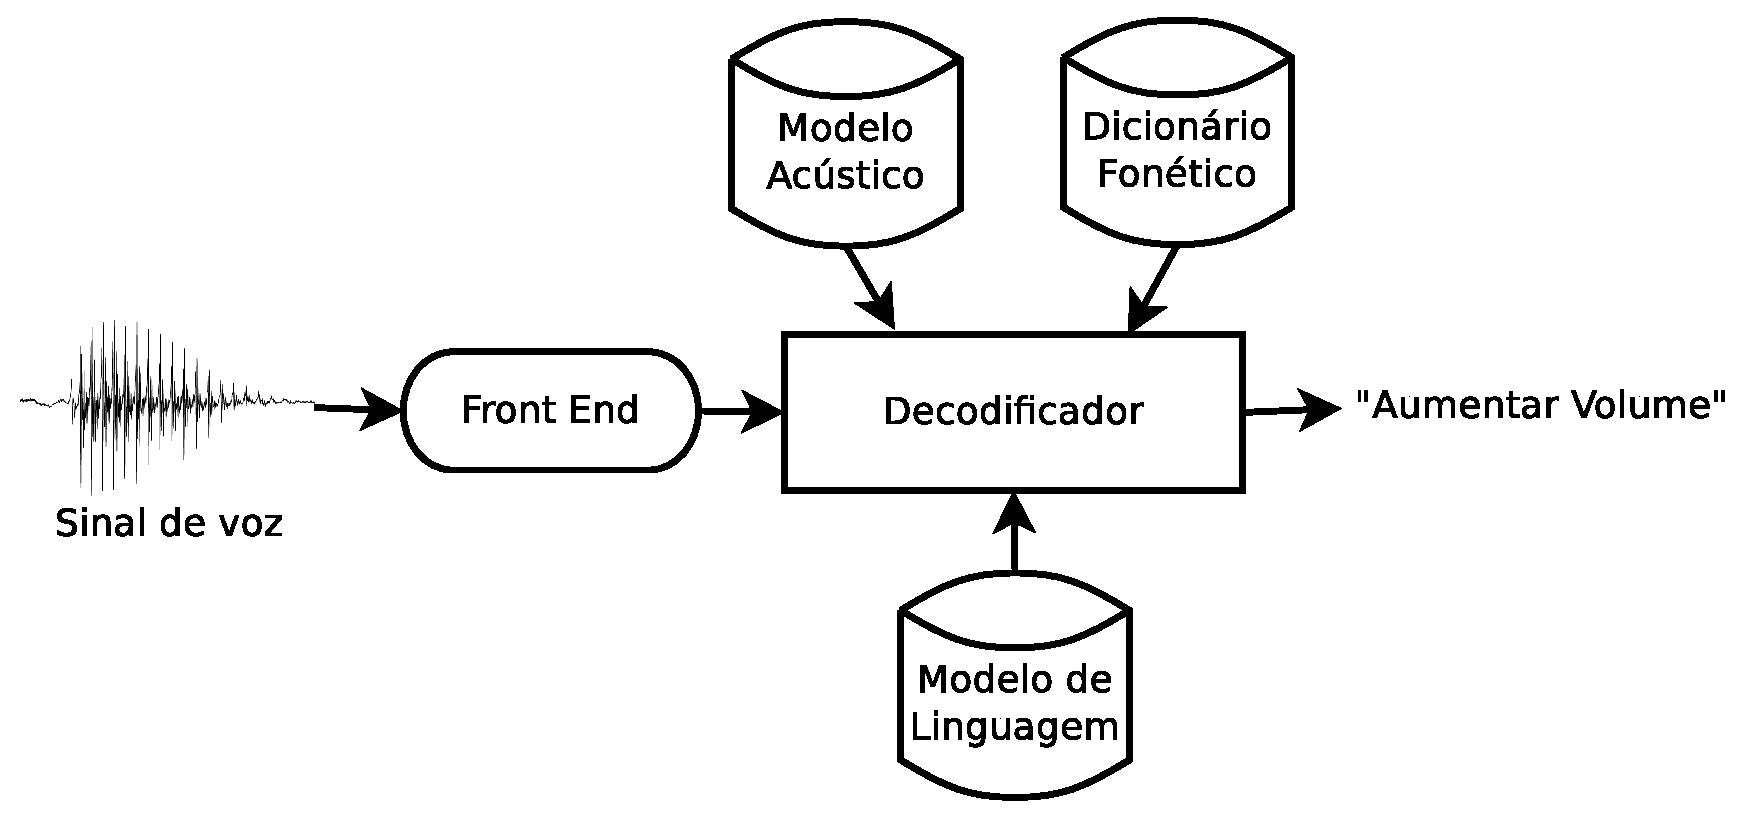
\includegraphics[width=.65\textwidth]{Figures/asr_sch}
	\caption{Esquem�tico de um sistema ASR}
	\label{fig:asr_sch}
\end{figure}

% http://andicelabs.com/2014/03/usb-audio-beaglebone/
Como sa�da anal�gica do sistema TTS, a voz sintetizada deve ser reproduzida por
um dispositivo externo � BeagleBone, j� que esta n�o possui alto-falantes
pr�prios. Como visto em~\cite{andicelabs}, o dispositivo prim�rio de sa�da de
�udio � o HDMI, o qual pode ser desabilitado mediante modifica��es
em par�metros do \textit{kernel}. Feito isso, o USB, que � o dispositivo secund�rio, se
torna o principal, fazendo com que a solu��o mais simples seja plugar um 
alto-falante (\textit{speaker}) na porta USB.
Na p�gina oficial do eSpeak, um arquivo de cabe�alho (\textit{header}) permite a
utiliza��o de uma API em C/C++, a qual facilita o acesso aos m�dulos do 
\textit{software} que permitem que a BBB ``fale''~\cite{eSpeak}.

%% http://arduino.cc/en/Tutorial/SimpleAudioPlayer
%% http://www.instructables.com/id/Simple-Wav-Player-Using-Arduino/?lang=pt&ALLSTEPS
%% http://forum.arduino.cc/index.php?topic=49654.0 -- can arduino talk without shield?
%% http://www.instructables.com/id/Twitter-Enabled-Text-to-Speech/
%Links �teis podem ser encontrados em~\cite{arduino_player}
%e~\cite{instructables_player}, os quais ensinam o passo-a-passo para o projeto e
%constru��o de um circuito amplificador. 

\subsection{Compara��o entre Plataformas}
A escolha da plataforma foi fundamental para a esquematiza��o do projeto.
Arduino, Raspberry Pi e BeagleBone Black foram as tr�s principais op��es a
serem escolhidas. Diversos tutoriais de compara��o entre as plataformas foram
consultados e est�o dispon�veis na Internet~\cite{mhl,randomnerd,makezine}.
O Arduino, apesar de ser uma ferramenta flex�vel e com grande capacidade de
interfaceamento com uma vasta quantidade de dispositivos, � uma plataforma
simples, recomendada para projetos de menor porte. O microcontrolador, que pode 
ser programado em C, torna-se muito limitado quando o projeto requer um servidor
est�vel e relativamente potente.
J� o Raspberry Pi, por ser bastante completo, enquadra-se no conceito de 
mini computador, sendo necess�rio a instala��o de um sistema operacional. Todo 
o seu armazenamento � fornecido por um cart�o SD, al�m de ser poss�vel
conect�-lo � Internet atrav�s de um conector Ethernet. O Raspberry Pi possui 
ainda uma interface de sa�da HDMI e � bastante �til para aplica��es gr�ficas.

\begin{table}[!h]
\centering
\caption{Compara��o entre as tr�s principais plataformas}
\label{comparison}
\begin{tabular}{c|c c c}
\hline
				& Arduino UNO & BeagleBone Black & Raspberry Pi \\
\hline
Chip			& -          & TI AM3359              & BCM2835 \\
CPU				& ATMega328  & ARM Cortex-A8          & ARM1176JZ-F \\
CPU Freq.		& 16 MHz     & 1 GHz                  & 700 MHz \\
GPU				& -          & PowerVR SGX530         & Dual Core VideoCore IV \\
Mem�ria. RAM	& 2 kB SRAM  & 512 MB DDR3            & 512 MB SDRAM \\
Armaz. Flash	& 32 kB      & 2 GB eMMC, MicroSD     & SD, MMC, SDIO card slot \\
Pinos			& 14         & 65                     & 8 \\
Video			& -          & mini HDMI              & HDMI \\
Sistema Op.		& -          & Linux                  & Linux \\
Amperagem		& 42 mA      & 210-460 mA             & 150-350~mA \\
Voltagem		& 7-12 V     & 5 V                    & 5 V \\
USB				& -          & 1 Host, 1 Mini Client  & 2 Hosts, 1 Micro Power\\
Ethernet		& -          & 1 10/100 Mbps          & 1 10/100 Mbps \\
\hline
\end{tabular}
\end{table}

A BeagleBone Black � compar�vel ao Raspberry Pi. Entretanto, por ter mais pinos
(GPIO) e um processador mais poderoso, a plataforma � uma escolha �bvia para
projetos mais elaborados. Al�m de possuir diversas op��es de conex�o, a
BBB une a flexibilidade de interfaceamento do Arduino com a capacidade
de processamento r�pido do Raspberry Pi. Apesar da desvantagem no pre�o, n�o
restaram muitas d�vidas no momento da escolha dessa plataforma para o projeto.
Uma compara��o entre os principais par�metros dos tr�s equipamentos � dada na
Tabela~\ref{comparison}.

% Thiago: LIRC

\subsection{Protocolos de Comunica��o via Luz Infravermelha}
O funcionamento de controles remotos, com �nfase nos baseados em luz
infravermelha para televisores, � explicado de de forma clara e detalhada em
diversos tutoriais para ``curiosos'' dispon�veis na Internet, como os da revista
Mundo Estranho~\cite{mundoestranho} e do blog \textit{How Stuff Works?} da
UOL~\cite{uol_hsw}. Atualmente, a maioria dos aparelhos eletr�nicos recebe
informa��o atrav�s de sensores infravermelhos localizados em pain�is frontais.
Entretanto, devido � interfer�ncia que surge com a vasta transfer�ncia de
informa��o via IR, a comunica��o entre o controle remoto e a
televis�o ocorre geralmente em 4 passos: um comando \textit{start} inicia a
transfer�ncia, seguido dos bits do comando espec�fico (como aumentar o volume,
por exemplo) e do endere�o do aparelho. Por fim, um comando de \textit{stop}
encerra o envio de bits. Dessa forma, a chance de a informa��o ser reconhecida
por mais de um aparelho � baixa (salvo o caso de serem dois equipamentos do
mesmo tipo e da mesma empresa).

Uma das grandes dificuldades relacionadas ao controle de equipamentos
eletr�nicos � que os 4 passos acima s�o apenas uma forma gen�rica de
descrever a comunica��o, ou seja, cada empresa praticamente segue o seu pr�prio
padr�o para estabelecer a comunica��o entre os dispositivos: o n�mero, a ordem e
o significado dos bits � variado, a modula��o e codifica��o usada s�o diferentes
e a frequ�ncia dos pulsos pode oscilar entre 32~kHz e 42~kHz, chegando a 50~kHz
em determinados aparelhos mais modernos. Al�m disso, t�o rara quanto o
seguimento de uma comunica��o IR padronizada � a disponibiliza��o de
documenta��o pelos fabricantes, que tamb�m � bastante escassa. 

Neste trabalho, ser�o detalhados protocolos de duas fabricantes: RC-6 e sua 
vers�o pioneira RC-5, ambos da Philips; e o protocolo utilizado pela Samsung. 

\subsubsection{O Protocolo da Philips: RC-5 e RC-6}
A Philips utiliza seu pr�prio protocolo de comunica��o, chamado RC-5. A �ltima
documenta��o foi liberada em 1992, quando ainda n�o existiam muitos dos
equipamentos eletr�nicos atuais, como \textit{home theaters} ou DVDs. 

\begin{figure}[!h]
	\centering
	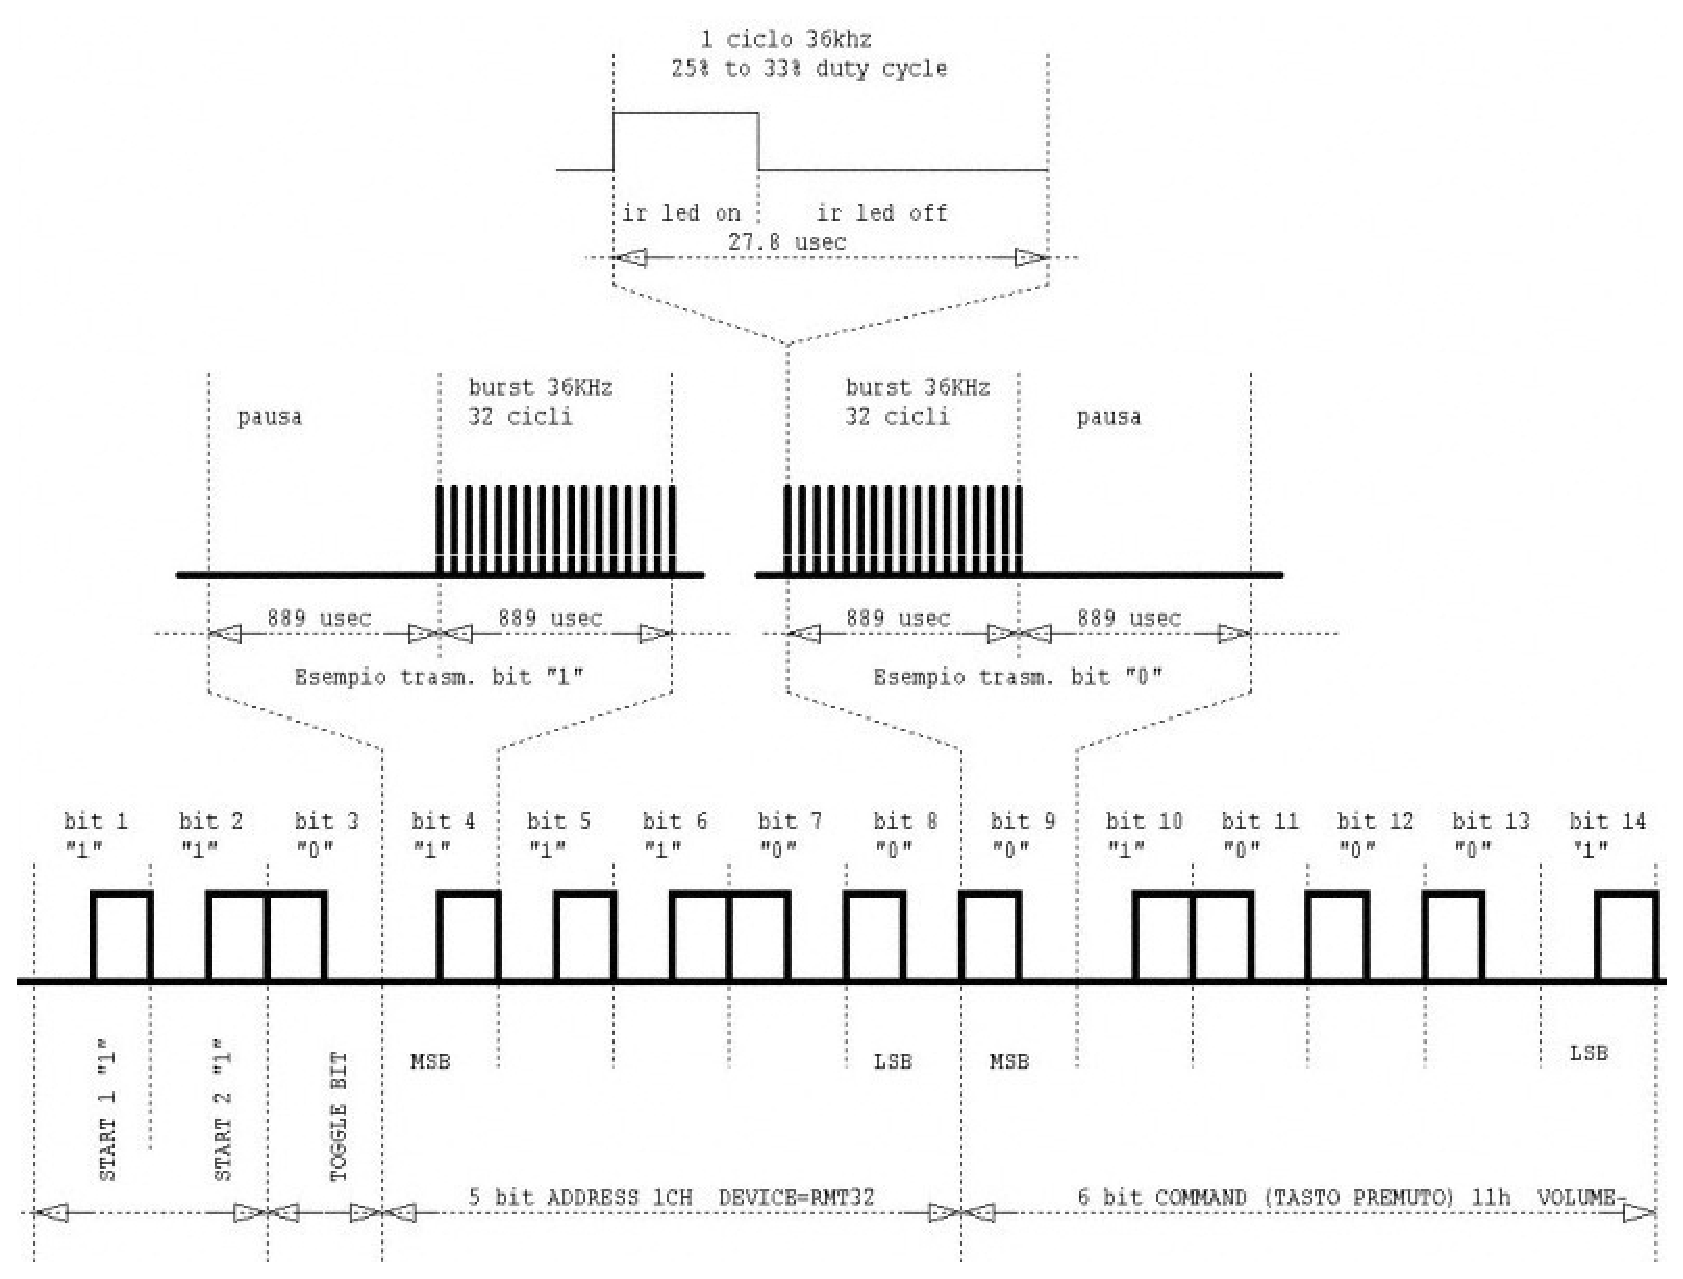
\includegraphics[width=.88\textwidth]{Figures/sch_rc5}
	\caption{Esquem�tico do protocolo RC-5 da Philips.}
	\label{fig:rc5}
\end{figure}

Nesse padr�o, os bits s�o codificados de acordo com o c�digo de Manchester, onde
cada bit, transmitido dentro de um per�odo fixo, � representado por uma
transi��o \textit{high-to-low} (0) ou \textit{low-to-high} (1). Esses padr�es de
dados s�o obtidos atrav�s de uma opera��o do tipo XOR (OU-Exclusivo) realizada
entre o clock do dispositivo e o dado propriamente dito~\cite{rc5}.

A Figura~\ref{fig:rc5} mostra a informa��o referente ao comando ``diminuir
volume'' contida num vetor de 14 bits. Os 11 �ltimos bits definem o endere�o do
aparelho de destino e o comando em si. Pode-se observar que qualquer bit �
representado por duas partes, sendo uma metade em n�vel baixo e a outra, em
n�vel alto. Cada n�vel ocorre num intervalo de 32 per�odos. O protocolo utiliza 
a modula��o por largura de pulsos (\textit{pulse width modulation} ou PWM). O 
n�vel alto � gerado por um PWM de \textit{duty cycle} que varia entre 25\% e
33\% do per�odo do pulso. Essa percentagem define o tempo em que o IR LED
permanece aceso, ou seja, no n�vel alto, o IR LED permanece ligado por per�odo
de $0,25\times1/36000~s$ e desligado por $0,75\times1/36000~s$, sendo o processo
repetido 32 vezes. A economia de energia � mostrada como justificativa para
explicar o motivo de o led piscar ao inv�s de se manter aceso por 100\% do
per�odo do pulso.

\begin{figure}[!h]
	\centering
	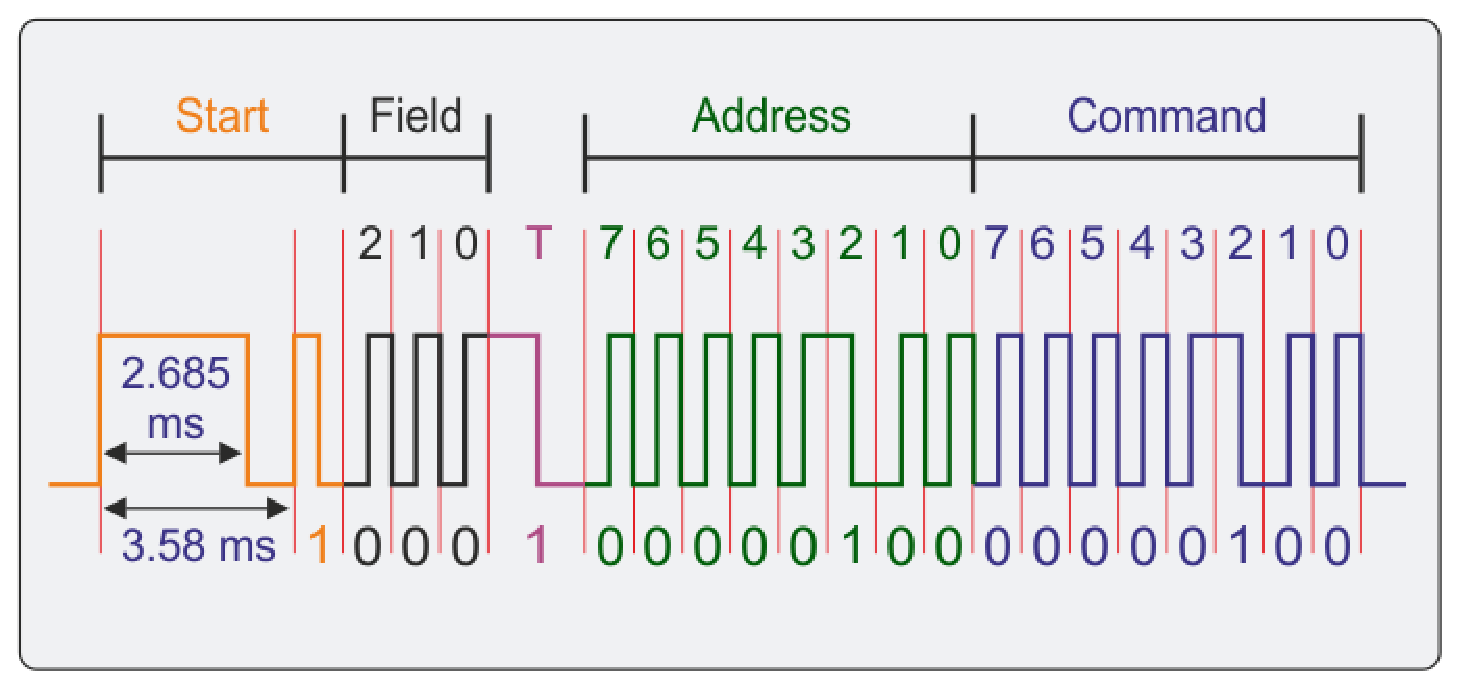
\includegraphics[width=.65\textwidth]{Figures/rc6}
	\caption{Esquem�tico do protocolo RC-6 da Philips.}
	\label{fig:rc6}
\end{figure}

Os aparelhos mais novos j� implementam a vers�o atualizada desse protocolo,
chamado de RC-6. Embora a Philips n�o tenha disponibilizado qualquer
documenta��o sobre este protocolo, h� f�runs na Internet que, atrav�s da
aplica��o de engenharia reversa, conseguem descrever o padr�o utilizado na
constru��o do sinal. Pela Figura~\ref{fig:rc6}, � f�cil notar que a quantidade
de bits carregada pelo sinal (em compara��o com o RC-5) aumentou de 14 para 22.
O c�digo Manchester tamb�m aparece invertido, j� que valor l�gico alto passa
agora a ser representado pela transi��o \textit{high-to-low} (1), enquanto o
valor baixo � definido por uma mudan�a \textit{low-to-high} (0). O primeiro bit
de \textit{start} tem uma dura��o maior, para garantir o ganho do AGC
(\textit{Automatic Gain Controller}) no circuito receptor; j� o segundo, tamb�m
de \textit{start}, � sempre mantido em valor alto para sincroniza��o. O bit de 
\textit{toggle}, o qual muda de estado caso uma tecla deixe de ser pressionada,
tamb�m possui uma dura��o mais longa do que os outros bits comuns. O per�odo de
um bit passa de 32 para 16 pulsos, exceto para os casos especiais (AGC e
\textit{toggle}). Por fim, os �ltimos 16 bits representam o endere�o do aparelho
e o referido comando a ser transmitido, respectivamente.

\subsubsection{O Protocolo da Samsung}
Assim como a Philips, a Samsung tamb�m utiliza seu pr�prio padr�o para
comunica��o entre os controles e os dispositivos eletr�nicos, o qual n�o
possui uma nomenclatura espec�fica. Felizmente, o documento de
\textit{application notes} do microcontrolador S3F80KB~\cite{S3F80KB} presente
em controles da Samsung encontra-se dispon�vel na Internet. O
protocolo define uma sequ�ncia de 34 bits, onde ambos os valores 0 e 1 s�o
representados por uma mudan�a no estado e diferenciados pela dist�ncia entre o
n�vel baixo dos pulsos.  Antagonicamente ao c�digo Manchester, onde a ordem da
transi��o define o valor do bit, o protocolo da Samsung sempre define os estados como
uma transi��o \textit{high-to-low}, na qual � estabelecida uma dura��o de
560~$\mu$s para o n�vel alto e duas para o n�vel baixo: 1690~$\mu$s para o bit
`1' e 560~$\mu$s para o bit `0'.

O n�vel alto do pulso dos bits normais � caracterizado por um PWM com 
frequ�ncia de 37,9~kHz e \textit{duty cycle} que pode variar entre 33\% e 50\% 
do per�odo do pulso.  Aproximadamente 21 pulsos na frequ�ncia portadora resultam
na dura��o de 560~$\mu$s.
O primeiro bit, chamado de \textit{leader}, tem dura��o mais longa para garantir 
o ganho no circuito receptor: 4,5~ms no n�vel alto e 4,5~ms no n�vel baixo; os
16 bits seguintes s�o divididos em dois blocos exatamente iguais de 8 
\textit{custom} bits cada; outras duas sess�es de 8 bits definem o bloco de
dado, onde o segundo bloco � o complemento dos bits do primeiro, o qual define
os dados propriamente ditos; o 34$\degree$ e �ltimo bit � sempre baixo e encerra
o comando.

\begin{figure}[!h]
	\centering
	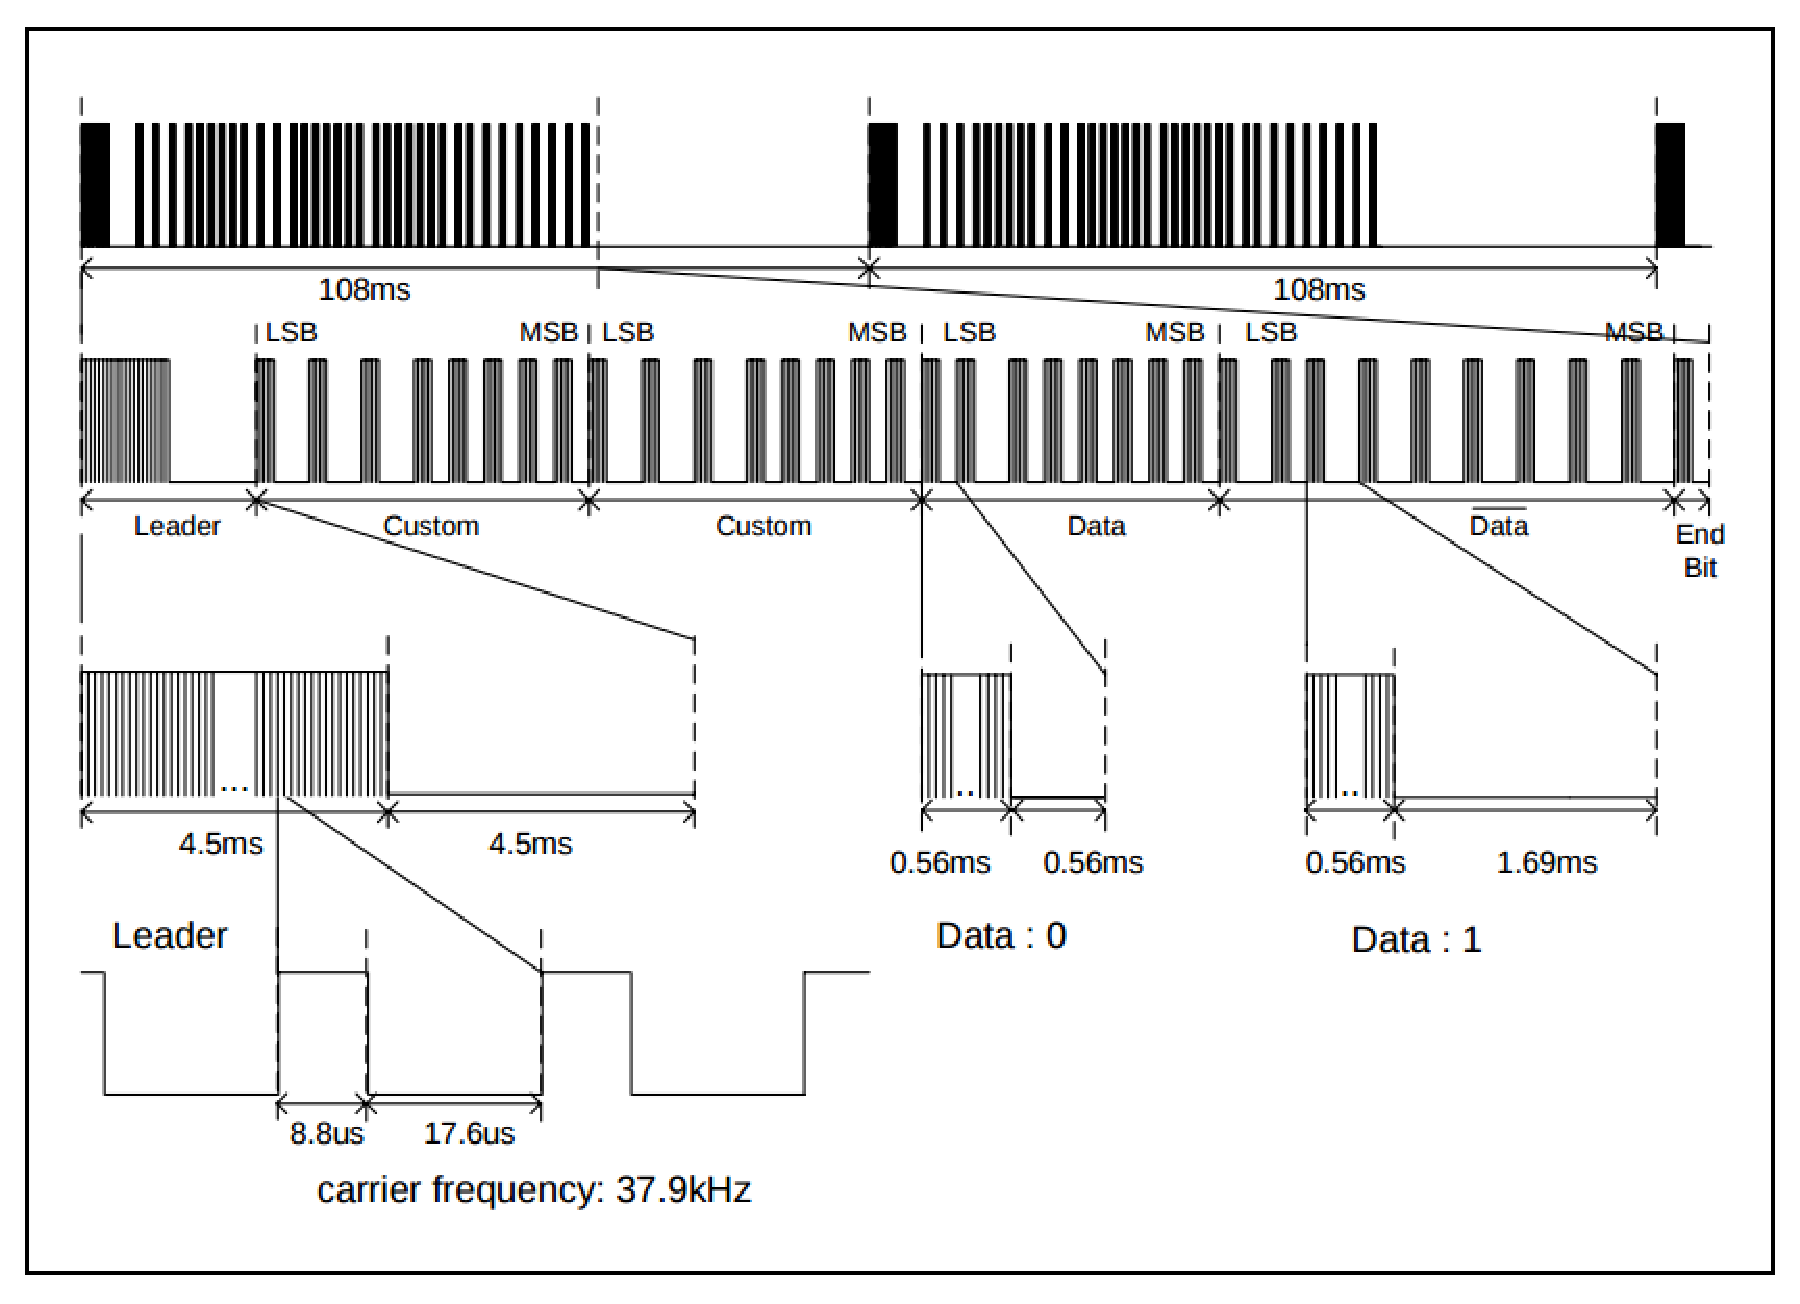
\includegraphics[width=.75\textwidth]{Figures/samsung_protocol}
	\caption{Esquem�tico do protocolo da Samsung.}
	\label{fig:samsung}
\end{figure}

\subsection{Produtos Relacionados}
Existem alguns produtos dispon�veis no mercado com a finalidade de tornar o
controle de equipamentos eletr�nicos mais pr�tico. Um deles � o Harmony Smart 
Control~\cite{harmonysc}, o qual possui em seu ``pacote'' um aplicativo para 
\textit{smartphones} iOS e Android (sem vers�o para tablets, todavia), um
\textit{hub} e um controle remoto gen�rico. Segundo a revis�o da CNET, vale a
pena pagar US\$ 130 por todas as funcionalidades que o sistema apresenta, como
usar uma conex�o de r�dio-frequ�ncia entre o \textit{smartphone}/controle com o
\textit{hub} (que, infelizmente, ainda n�o conseguiu se livrar do t�o antiquado
infravermelho), o que faz com que o usu�rio n�o precise apontar o controle para
o dispositivo que precisa controlar. Todavia, o \textit{hub} precisa estar numa
boa posi��o para conseguir emitir a informa��o de forma clara para o aparelho
desejado.

IRdroid � outro aplicativo que permite o controle de aparelhos televisivos com o
celular~\cite{irdroid}. Como o pr�prio nome sugere, funciona apenas em
dispositivos Android, desde que seu m�dulo de \textit{hardware} esteja acoplado 
na sa�da de audio \textit{jack} do \textit{smartphone}. Vers�es mais recentes 
j� possuem o \textit{hardware} que pode ser acessado via \textit{bluetooth}, 
custando US\$ 60 o mais caro. A grande vantagem � que o IRdroid, al�m de ser 
baseado na biblioteca LIRC, a qual possui uma vasta quantidade de equipamentos 
em seu banco de dados, possui c�digo livre e dispon�vel.

% Thiago: myuremote

Outras diversas solu��es s�o aplicadas apenas � \textit{smart TVs}, onde a
informa��o de controle � transmitida por \textit{wifi}. Nenhuma das aplica��es
encontradas para TVs convencionais possui suporte � reconhecimento e s�ntese de
voz \textit{offline} em PT\_BR.
\end{section}
%%% EOF %%%


% Metodologia ------------------------------------------------------------------
\begin{section}{Metodologia}
O servidor, por ser o elemento chave na consolida��o do projeto, deve ser o 
m�dulo a ser prioritariamente configurado, a fim de ser preparado para atender
�s devidas requisi��es, bem como executar qualquer tipo de aplica��o solicitada.
Sendo assim, a instala��o do sistema operacional Debian foi tomada como primeiro
passo, visto que houveram muitos problemas na instala��o do Ubuntu e do 
Angstrom. As depend�ncias a serem instaladas s�o mostradas na 
Lista~\ref{lst:dependences}.

� importante ressaltar que os sistemas operacionais embarcados s�o
simplifica��es de sistemas operacionais mais robustos, tendo a maior parte das
suas funcionalidades reduzidas ou simplificadas para se adequar � uma plataforma
de menor porte. Por isso, a prepara��o deve ocorrer a partir dos pacotes mais
b�sicos, como o GCC, por exemplo. Outros pacotes devem ser instalados de forma
gradual, tais quais os requeridos pelo Julius, eSpeak e os necess�rios para a
implementa��o do servidor LAMP em C.

\begin{lstlisting}[language=bash, caption={Pre-instala��o de depend�ncias no
servidor}, label={lst:dependences}]
# general dependences
build-essential alsa-tools alsa-base alsa-utils sox

# eSpeak dependences
libespeak-dev libportaudio2 libportaudio-dev

# Julius dependences
libasound2 libasound2-dev 

# LAMP dependences
apache2 libapache2-mod-fastcgi # apache server
mysql-server libapache2-mod-auth-mysql php5-mysql # MySQL
libmysqlclient-dev # C
phpmyadmin # (opcional?)
\end{lstlisting}

\subsection{Entrada de �udio e Reconhecimento de Voz}
Em~\cite{Cassio14}, o Julius foi configurado para funcionar em modo servidor
atrav�s da op��o nativa ``-adinnet'' (A/D \textit{Input from Network}, convers�o 
A/D com entrada pela rede). Isso permite que o Julius receba amostras de �udio
via \textit{streaming} atrav�s de uma comunica��o com um cliente gen�rico via
\textit{socket}. O c�digo foi alterado para que o resultado gerado pelo Julius,
tamb�m conhecido como senten�a, seja retornado ao cliente atrav�s desse mesmo
\textit{socket}. Al�m disso, uma aplica��o foi constru�da sobre a plataforma
Android exclusivamente para se comunicar com o servidor. Basicamente, as 
amostras de �udio obtidas pelo microfone do aparelho s�o enviadas, enquanto s�o
paralelamente analisadas a fim de se detectar o sil�ncio do fim da fala do
usu�rio. Feito isso, o aplicativo apenas aguarda a senten�a a ser enviada pelo
servidor.

A constru��o do dicion�rio fon�tico para o PT\_BR se d� por meio do
\textit{software} \texttt{lapsg2p}, o qual recebe uma lista de palavras como
entrada e gera suas transcri��es fon�ticas, conforme visto na lista abaixo, �
direita. J� a gram�tica � utilizada para restringir o vocabul�rio, de modo a
gerar somente uma das sente�as listadas, como mostrado na lista abaixo, �
esquerda. A constru��o da gram�tica no formato do Julius utiliza diretamente o
dicion�rio fon�tico em seu escopo.

\begin{minipage}[t]{.50\textwidth}
\begin{lstlisting}[label={lst:gram}]
<s> aumentar volume </s>
<s> diminuir volume </s>
<s> canal mais </s>
<s> canal menos </s>
<s> ligar televis�o </s>
<s> desligar televis�o </s>
<s> cadastrar controle </s>
<s> selecionar controle </s>
\end{lstlisting}
\end{minipage}
\begin{minipage}[t]{.50\textwidth}
\begin{lstlisting}[label={lst:dict}]
aumentar	a u~ m e~  t a X  
diminuir	dZ i~ m i~ n u j X  
volume		v o l u~ m i  
canal		k a n a w  
mais		m a j s
menos		m e~ n u s
televis�o	t e l e v i z a~ w~   
...
\end{lstlisting}
\end{minipage}

% http://stackoverflow.com/questions/2661129/espeak-sapi-dll-usage-on-windows
%A proposta do trabalho � adicionar funcionalidades ao c�digo do Julius,
%permitindo a produ��o de voz sintetizada atrav�s da incorpora��o da API do 
%eSpeak e a transmiss�o de informa��o para a TV atrav�s de um led IR conectado
%a um GPIO. Um sensor IR ficar� encarregado de receber informa��es de diferentes
%controles remotos para que sejam guardadas como registros no banco de dados.

%Toda a organiza��o do trabalho, bem como a comunica��o entre os membros sobre os
%passos tomados no decorrer do trabalho ser� feita atrav�s da plataforma
%Trello~\cite{trello}.\\

\subsection{An�lise do Sinal IR}
O controle RC2954201/01 da TV Philips 39PFL3008D/78 foi usado como base para a 
an�lise do sinal emitido. Inicialmente, um arduino UNO fui utilizado para
verificar o tempo em que o IR led permanecia ativo e inativo, armazenando-o em
uma matriz de duas colunas, como visto no Ap�ndice~\ref{app:arduino}. O Octave
foi utilizado para converter a matriz em um vetor �nico, no qual os �ndices
�mpares representavam o tempo de dura��o do modo \textit{burst} do IR led e as
posi��es pares, o tempo em que o IR led permanecia \textit{idle} (Vide
Ap�ndice~\ref{app:matlab}). Sendo assim, o vetor no qual as dura��es dos n�veis
altos e baixos alternam-se entre si foi convertido para uma forma de onda
quadrada, semelhante � mostrada na Figura~\ref{fig:rc6}.  A
Figura~\ref{fig:cmds} mostra a forma de onda quadrada para 4 bot�es diferentes
pressionados de forma n�o consecutiva. Pode-se notar que os sinais s�o
exatamente iguais at� aproximadamente $t=15ms$, onde come�am a ser exibidos os
bits referentes ao comando espec�fico. J� na Figura~\ref{fig:vol+}, o bot�o
``volume mais'' foi pressionado por quatro vezes consecutivas. Percebe-se que os
sinais s�o completamente id�nticos, exceto o bit de \textit{toggle}, o qual muda
sempre que um bot�o � solto.

\begin{figure}[!h]
	\centering
	\includegraphics[width=\textwidth]{Figures/cmds}
	\caption{Mudan�a nos bits de comando ap�s pressionar N�O consecutivamente 
			4 bot�es diferentes.}
	\label{fig:cmds}
\end{figure}

\begin{figure}[!h]
	\centering
	\includegraphics[width=\textwidth]{Figures/volume+}
	\caption{Mudan�a no bit de \textit{toggle}(T) ap�s pressionar o bot�o 
			``volume+'' por 4 vezes consecutivas.}
	\label{fig:vol+}
\end{figure}

\subsection{Banco de Dados MySQL}
Como o sistema foi projetado para, futuramente, dar suporte ao controle de 
diversos aparelhos eletr�nicos, a ado��o de um banco de dados foi vista como 
solu��o para facilitar o acesso a uma maior variedade de dispositivos e, assim,
tornar o projeto um sistema de prop�sito mais geral. Al�m disso, a seguran�a
dos dados, que ser�o constantemente manipulados, ser� mantida, podendo estes ser
recuperados apenas olhando para o banco. %(????)

Inicialmente, apenas a entidade TELEVIS�O foi criada, onde uma
tabela intitulada ``TV'' cont�m atributos como a marca do aparelho e os comandos
a serem transmitidos, como visto na Tabela~\ref{tab:tv}. Com isso,
quaisquer campos podem ser satisfatoriamente acessados atrav�s de um simples
c�digo SQL (como o mostrado abaixo). %a fim de se montar um determinado comando.
Assim, podemos recuperar os bits de refer�ncia e, posteriormente, decodific�-los
de acordo com o protocolo do aparelho para, finalmente, enviar para o led IR.

\begin{lstlisting}[style=code, language=sql]
SELECT campo FROM TV WHERE marca='marca_da_tv' 
\end{lstlisting}

O acesso ao banco de dados � inteiramente intermediado pela linguagem C. Para 
tal, uma biblioteca especial chamada \texttt{mysql.h} foi utilizada, na qual as
\textit{queries} s�o realizadas pela passagem de um comando SQL como uma
\textit{string} (Vide Ap�ndice~\ref{app:lamp}).

\begin{table}[h]
\centering
\caption{Tabela TV}
\label{tab:tv}
\begin{tabular}{c|ccccc}
\hline
Marca   & volume+  & volume-  & canal+   & canal-   & ligar    \\ 
\hline
Lg      & 10111011 & 11110110 & 11000010 & 00010111 & 01011111 \\
Sony    & 11110110 & 01011111 & 00011111 & 10111011 & 11000000 \\
Samsung & 00110111 & 11000010 & 11010000 & 11011110 & 11011100 \\
Philips & 00011111 & 10111011 & 11000000 & 11011010 & 11010111 \\ 
\hline
\end{tabular}
\end{table}

% Thiago: Detalhes sobre o que foi feito com o Arduino

\begin{subsection}{GPIO}
Como no Arduino, a BeagleBone possui muitos pinos de entrada e sa�da para 
diversas fun��es, algo que o Raspberry Pi carece. Os GPIOs (\textit{general
purpose input/output}, ou pinos de entrada e sa�da de prop�sito geral) podem ser
usados da forma mais conveniente ao desenvolvedor, sendo poss�vel controlar a
tens�o de sa�da, receber \textit{feedback} de sensores digitais e anal�gicos,
etc. De acordo com o \textit{datasheet}~\cite{am335x}, o processador possui 128
pinos de GPIO divididos em 4 m�dulos de 32 pinos cada. Por�m, o mapeamento
entre os pinos da BeagleBone Black e os do processador n�o � exatamente igual 
(da mesma forma que o n�mero dos pinos do Arduino UNO n�o equivale aos do
ATmega328, por exemplo). Portanto, � necess�rio saber como os pinos est�o
dispostos na placa.

%\begin{figure}[!h]
%	\centering
%	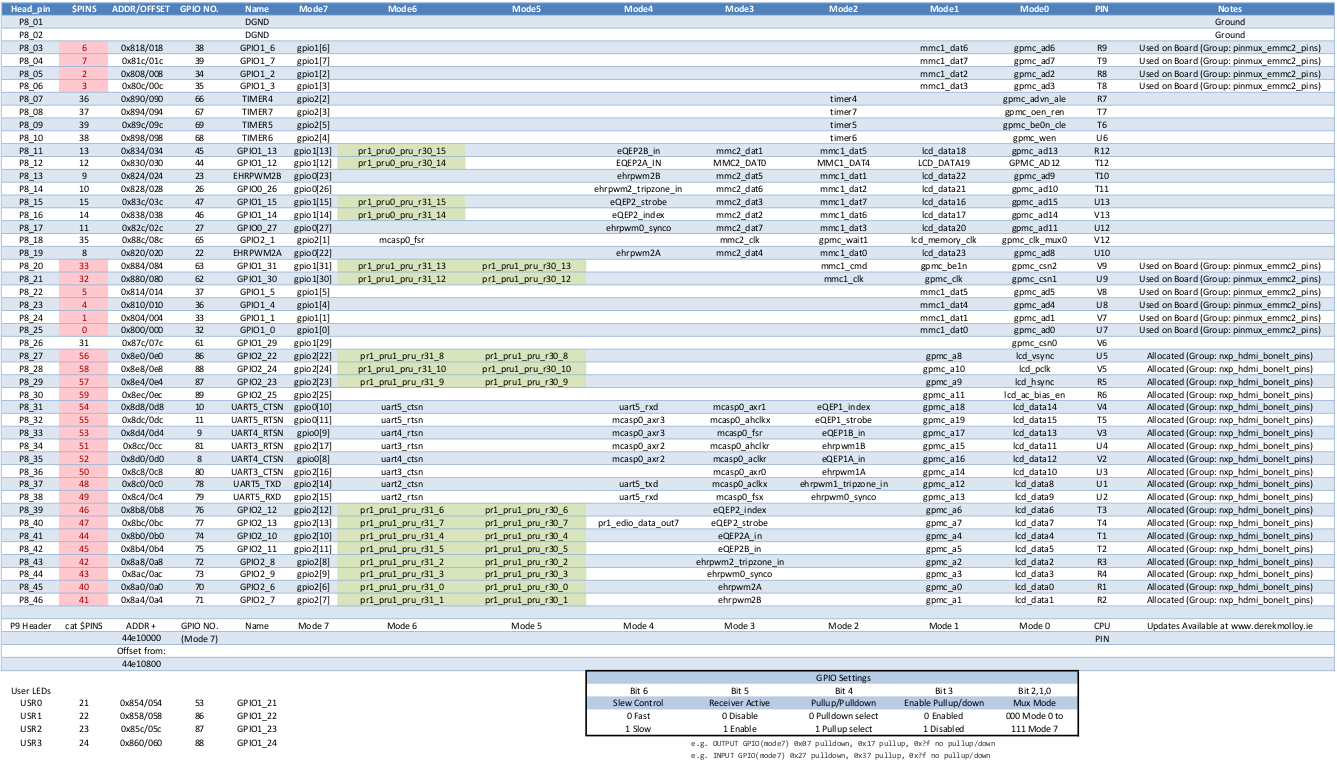
\includegraphics[width=\textwidth]{Figures/BBBp8}
%	\caption{Mapeamento de Pinos do Header P8 da BeagleBone}
%	\label{fig:BBBp8}
%\end{figure}

\begin{table}[h]
\centering
\caption{Mapeamento de Pinos do \textit{Header} P8 da BeagleBone}
\label{tab:BBBp8}
\begin{tabular}{cccccclc}
\hline
\textit{Head pin} & \$Pins & Endere�o & \textit{offset} & N$\degree$ GPIO & Nome & Modo7 & Pino \\ 
\hline \hline
 1,2 &   &       &     &    & DGND     &           &     \\
 3   & 6 & 0x818 & 018 & 38 & GPIO\_6  & gpio1[6]  & R9  \\
 4   & 7 & 0x81c & 01c & 39 & GPIO\_7  & gpio1[7]  & T9  \\ 
 5   & 2 & 0x808 & 008 & 34 & GPIO\_2  & gpio1[2]  & R8  \\ 
 6   & 3 & 0x80c & 00c & 35 & GPIO\_3  & gpio1[3]  & T8  \\ 
13   & 9 & 0x824 & 024 & 23 & EHRPWM2B & gpio0[23] & T10 \\
19   & 8 & 0x820 & 020 & 22 & EHRPWM2A & gpio0[22] & U10 \\
\hline
\end{tabular}
\end{table}

\begin{figure}[!h]
	\centering
	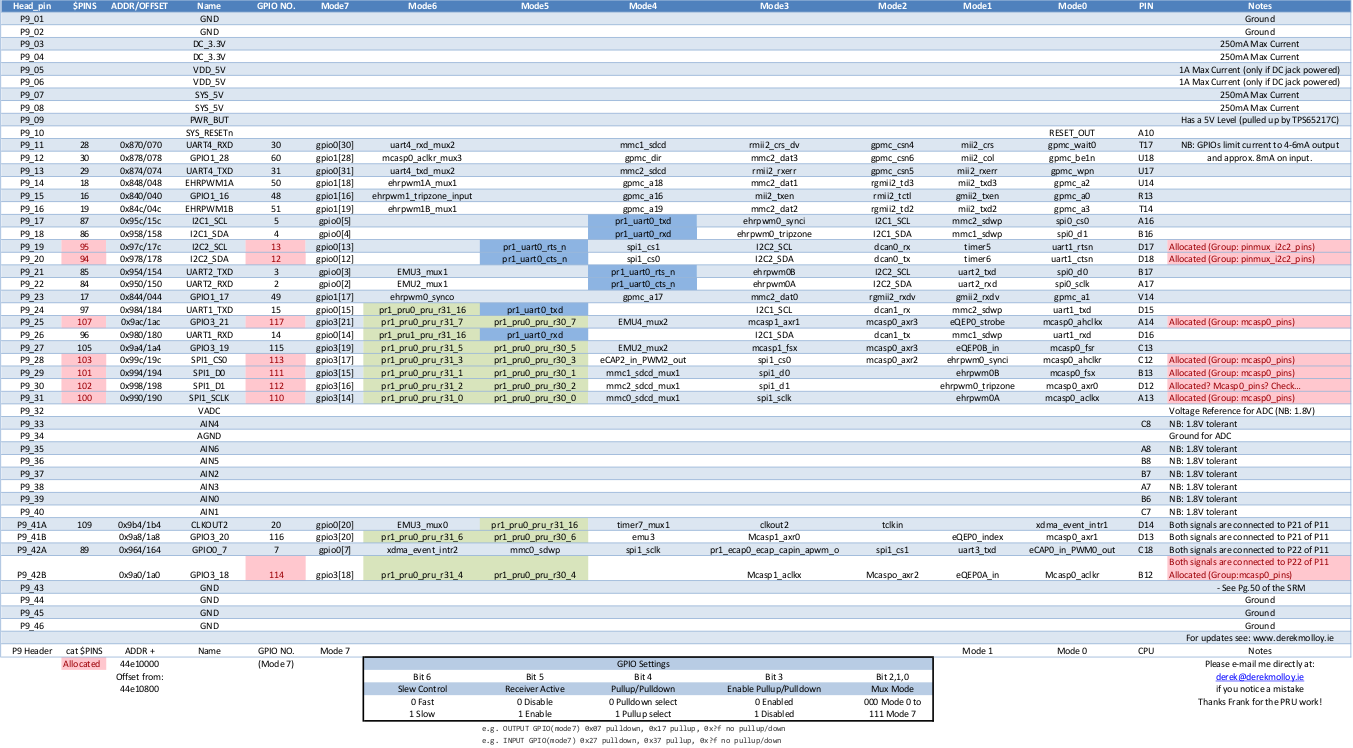
\includegraphics[width=\textwidth]{Figures/BBBp9}
	\caption{Mapeamento de Pinos do Header P9 da BeagleBone}
	\label{fig:BBBp9}
\end{figure}

Como o objetivo n�o � prototipar a partir do processador, o mapeamento correto 
dos pinos � crucial para conseguir alguma sa�da v�lida dos pinos da placa. 
% e sim usar a placa
%de desenvolvimento a qual possui pinos mais acess�veis. 
As Tabelas~\ref{tab:BBBp8} e~\ref{tab:BBBp9} mostram esse mapeamento.

Existem 3 formas de se acessar e controlar os pinos de GPIO, a primeira �
atrav�s da IDE web que vem instalada no Angstrom de f�brica, mas como o OS foi 
trocado pelo Debian essa op��o n�o � vi�vel. Outra forma, a mais complexa, �
iniciar o m�dulo e atribuir valores atrav�s de registradores, tal processo �
explicado no \textit{datasheet}~\cite{am335x}, mas despenderia muito tempo e
seria pouco port�vel. A �ltima solu��o foi introduzida com o kernel 3.8.x do
Linux embarcado, acessando as interfaces GPIO atrav�s do kernel, basicamente
atribuindo valores a arquivos. Tal processo s� pode ser executado como root,
ent�o deve se entender bem o que est� fazendo antes de executar tais comandos.

Os arquivos de configura��o do GPIO pelo kernel est�o localizados no caminho
\texttt{/sys/class/gpio}. Ao se modificar o arquivo \texttt{export}, o qual 
inicializa o pino, o diret�rio \texttt{gpiochipXX}, que cont�m os arquivos
necess�rios para a configura��o do pino, � criado. Apenas os arquivos
\texttt{direction} e \texttt{value} s�o necess�rios para a tarefa de piscar um
led, os quais indicam se o pino ser� de entrada ou sa�da e o valor que ser�
atribu�do ao pino, respectivamente.

\begin{lstlisting}[language=bash]
echo 51  > /sys/class/gpio/export # exporta o pino 51 / GPIO_19 / pino 16
echo out > /sys/class/gpio/gpiochip51/direction # define o pino como sa�da
for i in `seq 10`; do
	echo 1 > /sys/class/gpio/gpiochip51/value # seta o valor alto no pino
	sleep 1
	echo 0 > /sys/class/gpio/gpiochip51/value # seta o valor baixo no pino
	sleep 1
done 
echo 51 > /sys/class/gpio/unexport # libera o pino 51 / GPIO_19 / pino 16
\end{lstlisting}

%\begin{equation}
%	\text{GPIO Number on BBB} =  1 \times 32 + \text{GPIO Number on Mode7} \notag
%\end{equation}

Os comandos listados acima s�o o suficiente para piscar um led conectado ao
pino 51, ou pino 16 do \textit{header} P9.
\end{subsection}
\end{section}
%%% EOF %%%


% Or�amento --------------------------------------------------------------------
\begin{section}{Or�amento}
% BBB: http://www.farnellnewark.com.br/ : 270,55 + 36,80 = 307,35
% BBB: http://www.aliexpress.com.br/ : 180,34
% Rpi: http://www.aliexpress.com.br/ : 147,92
\begin{table}[!h]
\centering
\begin{tabular}{l|c c c c}
	\hline
	Produto & USD (U\$) & BRL (R\$) & IOF (R\$) & Total (R\$) \\
	\hline
	BBB &\\
	Smartphone &\\
	IR Led &\\
	IR Sensor &\\
	% Capacitor &\\
	% Resistor &\\
	USB Speaker 8~$\Omega$ &\\
	% LM386 amplifier&\\
	\hline
	Total & & & & 500 conto\\
\end{tabular}
\end{table}
\end{section}


% Dificuldades e Solu��es ------------------------------------------------------
\begin{section}{Dificuldades e Solu��es}
\begin{enumerate}
\item O �ngstr�m � o sistema operacional de f�brica da BeagleBone Black, %$^{\scriptsize{\textregistered}}$, 
bastante referenciado em f�runs e candidato 
principal para ser a base do projeto. Entretanto, o sistema e a nomenclatura de 
pacotes n�o correspondiam com os usados nas distribui��es Debian, o que 
impossibilitava a instala��o das depend�ncias necess�rias para o uso das 
ferramentas de processamento de voz. Al�m disso, o �ngstr�m tamb�m consumia 
muito espa�o de armazenamento na \textit{flash}, ocupando sozinho 1.6~GB de 2~GB 
por conta de sua interface gr�fica.

A op��o seguinte foi o Ubuntu, pois a similaridade do sistema de pacotes
\texttt{apt-get} com a distribui��o \textit{desktop} tornaria a integra��o mais
f�cil. Por�m, a instala��o da vers�o 14.04 tamb�m ocupava espa�o demais na
mem�ria \textit{flash}: aproximadamente 1.2~GB. Al�m do problema de espa�o,
outra dificuldade foi a conex�o com a Internet, j� que o acesso convencional ao
reposit�rio de pacotes n�o funcionava. 

A solu��o veio com a instala��o de um terceiro e �ltimo sistema operacional, o 
Debian 7.8 wheezy. Este se mostrou muito mais leve e ``enxuto'' em sua vers�o 
\textit{minimal}, ocupando menos de 500~MB da mem�ria. Al�m disso, todos os 
pacotes necess�rios para conex�o com a Internet funcionaram perfeitamente.

\item A BeagleBone Black n�o possui 
sa�da de �udio nativa, tampouco conectores do tipo \textit{audio jack}. No 
Debian, a sa�da padr�o de �udio � pelo conector HDMI, mas pode ser substitu�da 
pelo USB mediante modifica��es em par�metros do \textit{kernel}. O modo mais 
f�cil, considerando que redirecionar a sa�da do eSpeak para um GPIO seria muito 
trabalhoso, seria conectar um alto-falante USB � BeagleBone Black.
Em se tratando de um prot�tipo, um 
\textit{headphone} faz o papel de um alto-falante que deve consumir pouca 
energia e ter um tamanho limitado. Foi-se cogitada a constru��o de um circuito 
com um amplificador LM386 para o \textit{speaker}, por�m a obten��o de um D/A 
PCM2707 n�o custaria menos de US\$ 15.

\item A BeagleBone Black n�o possui 
conex�o \textit{wifi}. Al�m da dificuldade em atualizar o \textit{kernel} pra 
receber um \textit{shield/cape}, o mesmo teria de ser conectado na  porta USB, 
a qual j� estaria sendo usada pelo alto-falante. Portanto, a solu��o mais f�cil 
foi conectar um roteador \textit{wifi} � porta Ethernet da BBB atrav�s 
de um cabo UTP.

\item O c�digo criado para o Arduino faz um \textit{dump} da informa��o captada
pelo \textit{photosensor}, verificando o tempo que ele passa ligado e desligado
e salvando v�rias medidas de tempo numa matriz de inteiros, o que deixa o
armazenamento dessa informa��o pouco vi�vel. Ap�s traduzir o c�digo para que
seja executado na BBB, o ideal seria converter os valores de tempo para um
\textit{array} de bits (``110101010'', por exemplo) para que fosse mais f�cil
salvar no banco de dados. Isso j� funciona, por�m somente para o protocolo
RC-6.

\item A fun��o \texttt{mysql\_query()} recebe uma \textit{string} contendo o
comando SQL para acessar o banco de dados MySQL. Caso se queira editar o valor
de um atributo numa determinada tabela, por exemplo, basta passar o valor e o
atributo como par�metros para a fun��o, o que exige que as \textit{strings}
sejam manipuladas constantemente a fim de tornar as requisi��es autom�ticas.
Para que n�o se utilize mais espa�os de mem�ria do que necess�rio, optou-se pela
aloca��o din�mica atrav�s da fun��o \texttt{malloc()}, auxiliada pela fun��o
\texttt{sprintf()}, a qual � respons�vel pela jun��o de \textit{strings}. O
c�digo ainda est� sob revis�o, j� que diversas falhas de segmenta��o v�m
ocorrendo devido � erros no gerenciamento de mem�ria. Al�m disso, o custo
computacional provocado pelas diversas \textit{queries} no banco ainda n�o pode
ser previsto. Essa previs�o � muito importante visto que, em uma futura
utiliza��o de um servidor Apache para acesso remoto de qualquer lugar via
cliente PHP, por exemplo, o efeito \textit{snowball} pode surgir como uma
consequ�ncia negativa.

\item Como explicado na se��o~\ref{sec:rev_th}, um bit � representado por duas
partes, sendo uma metade n�vel baixo e a outra n�vel alto. Para o RC-6, cada 
n�vel ocorre num intervalo de 16 ciclos (ou 32 ciclos para no caso do protocolo
RC-5), sendo o n�vel alto gerado pelo protocolo por modula��o PWM com
\textit{duty cycle} m�nimo de 25\% do per�odo do ciclo, tal como o mostrado na
Figura~\ref{fig:bits}.

\begin{minipage}{\linewidth}
	\centering
	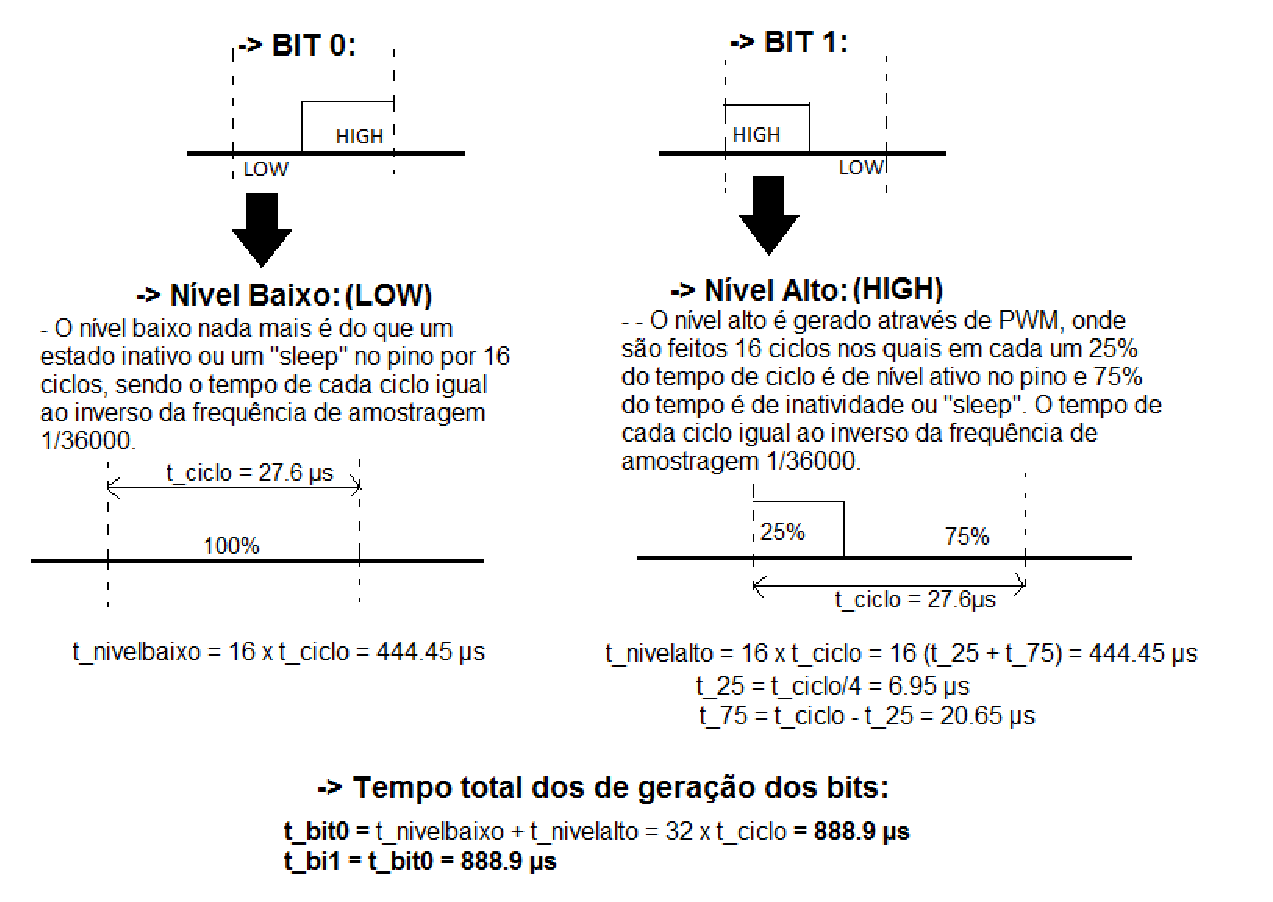
\includegraphics[width=.85\textwidth]{Figures/Bits}
	\captionof{figure}{Processo de gera��o de cada bit}
	\label{fig:bits}
\end{minipage}

Por�m, a BeagleBone Black leva um tempo de 42~$\mu$s para escrever HIGH no pino,
isto �, para gerar a parte ativa do PWM, a plataforma responde com um tempo 
maior do que o pr�prio ciclo, o qual demora 27.6~$\mu$s aproximadamente.
Levando-se em conta o tempo que a BeagleBone leva para escrever (chamado
de $t_{set}$), de acordo com o esquema mostrado na Figura~\ref{fig:ciclo_pwm},
a dura��o do bit seria de 111,6~$\mu$s.

\begin{minipage}{\linewidth}
	\centering
	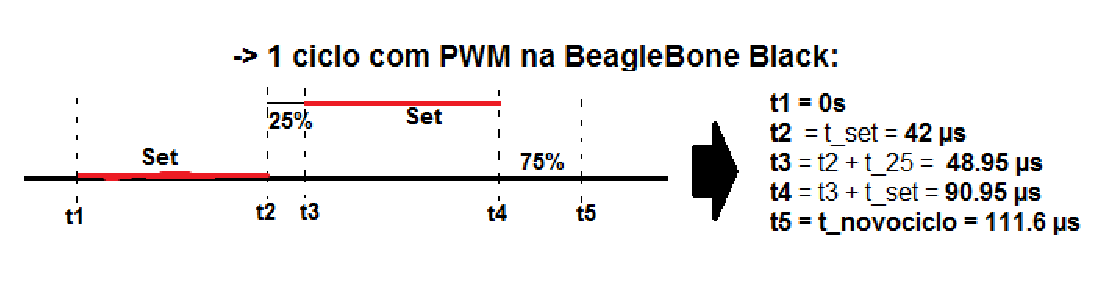
\includegraphics[width=.65\textwidth]{Figures/Ciclo_PWM}
	\captionof{figure}{Ciclo com PWM na BeagleBone Black}
	\label{fig:ciclo_pwm}
\end{minipage}

Logo, este novo tempo de ciclo ir\'{a} afetar diretamente na aquisi�\~{a}o dos dados,
pois reduzir\'{a} a frequ\^{e}ncia de amostragem e n\~{a}o ser\'{a} mais poss\'{i}vel
transmitir os comandos em infravermelho, fazendo uma conta de quanto ir\'{a} impactar,
tem se que:
\begin{equation}
	1 \ s \rightarrow 36k \ valores \rightarrow 27 \ \mu s/valor \notag
\end{equation}
\begin{equation}
	1 \ s \rightarrow n \ valores \rightarrow 111.6 \ \mu s/valor \notag
\end{equation}

Resolvendo a regra de 3 inversa, tem se:
\begin{equation}
	n \approx 8.96k \rightarrow f_{coding} = 8.96 \ kHz \notag
\end{equation}
\begin{equation}
	\frac{f_s}{f_{coding}} = \frac{36k}{8.96k} \approx 4 \notag 
\end{equation}

Com isso pode se observar que a frequ\^{e}ncia de amostragem seria 4 vezes menor
que a desejada. 

%Para combater este problema, foi necess\'{a}rio abrir m\~{a}o do PWM e reajustar
%como cada n\'{i}vel seria gerado, ent\~{a}o o n\'{i}vel alto (antes com PWM) passou a ser
%nada mais que o pino ativo pelo tempo de 1 ciclo ($t_{ciclo} = 27.6 \ \mu s$).
%
%\begin{minipage}{\linewidth}
%	\centering
%	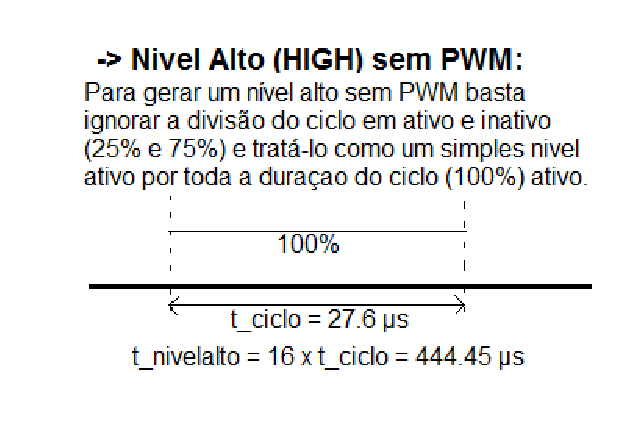
\includegraphics[width=.45\textwidth]{Figures/Bit_noPWM}
%	\captionof{figure}{N\'{i}vel alto sem o PWM}
%	\label{fig:bit_nopwm}
%\end{minipage}
%
%\begin{minipage}{\linewidth}
%	\centering
%	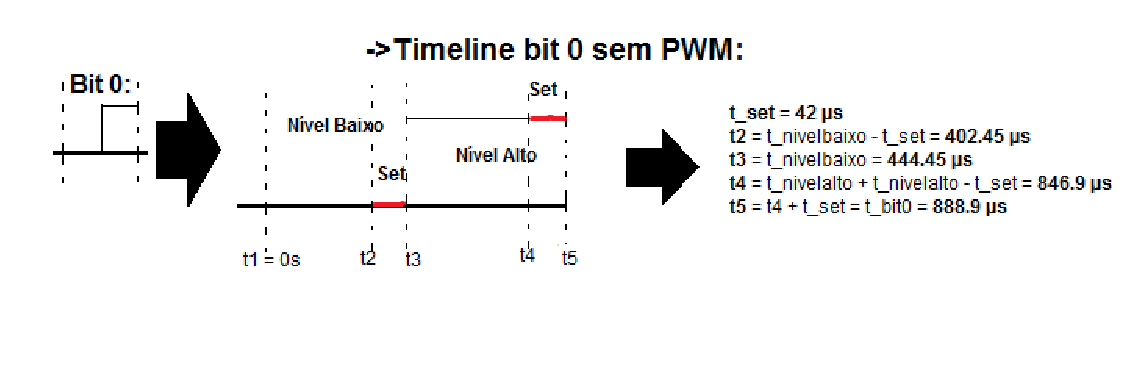
\includegraphics[width=.85\textwidth]{Figures/Bit0_Coding}
%	\captionof{figure}{Timeline do bit 0 na BeagleBone Black}
%	\label{fig:bit0_coding}
%\end{minipage}


%que usar diversas vezes aloca�\~{o}es de mem\'{o}ria (\textit{*malloc()}) e
%\textit{sprintf()}s, tornando o c\'{o}digo, em mais espec\'{i}fico o
%gerenciamento dos campos da mem\'{o}ria, ca\'{o}tico, apresentando algumas vezes
%falha de segmenta�\~{a}o. Posteriormente, com a adi�\~{a}o de outros aparelhos e
%mais tabelas, estas queries ficaram cada vez mais recorrentes e mais falhas
%poderam acontecer. 

%Al\'{e}m disso, por estarmos acessando o MySQL por meio de uma outra linguagem (no caso C), n\~{a}o podemos prever 
%agora poss\'{i}veis custos computacionais que essas diversas e constantes queries poder\~{a}o gerar nas threads 
%dentro do BeagleBone Black\textregistered. Numa poss\'{i}vel e vindoura utiliza�\~{a}o de um servidor Apache com o 
%PHP essa comunica�\~{a}o adicional e constante poder\'{a} resultar em significante custo computacional tornando-se um 
%efeito \textit{snowball}, bola de neve.
\end{enumerate}
\end{section}
%%% EOF %%%


% Trabalhos Futuros ------------------------------------------------------------
\begin{section}{Trabalhos Futuros}
De acordo com o relato dispon�vel em~\cite{nielsen04}: ``Dado que o meu home
theater � modesto, ele requer que eu consiga manejar `apenas' 6 controles
remotos para a simples tarefa de assistir a um filme''. Seria �timo se houvesse
um controle remoto universal que permitisse acesso � \emph{todos} os aparelhos 
do ambiente residencial, mesmo os que est�o em c�modos diferentes. Ter o controle
sempre consigo e poder us�-lo por uma tecnologia \textit{hands free} mesmo
quando estivesse fora de casa � um sonho de qualquer consumidor.

\begin{itemize}
	\item Expandir para v�rios aparelhos, tornando a BeagleBone um servidor
	centralizado no ambiente dom�stico. Isso tamb�m acarretar� em um n�mero 
	maior e mais complexo de tabelas no banco de dados, contendo os diversos 
	aparelhos e seus comandos;
	
	\item Em cada compartimento onde houvesse um aparelho eletr�nico a ser
	controlado, haveria um microcontrolador (a ser avaliado, preferencialmente 
	mais barato que o Arduino) capaz de controlar determinado(s) aparelhos;

	\item A BeagleBone e todos os outros microcontroladores estariam
	conectados � mesma rede LAN. Somente a BBB precisaria estar conectada � 
	Internet, de modo que n�o houvesse limita��o de dist�ncia para a conex�o 
	com o \textit{smartphone};
	
	\item Utilizar de forma eficiente o servidor Apache com o PHP, para que uma
	p�gina web seja criada e por meio dela informa��es de an�lise do sistema 
	possam ser guardadas e acessadas remotamente pelo desenvolvedor, para que 
	haja um algoritmo de detec��o e an�lise de problemas mais eficiente ao 
	usu�rio. Essa nova funcionalidade tamb�m poder� disponibilzar um registro 
	das atividades do usu�rio com o sistema, podendo ficar dispon�vel para
	monitoramento em \textit{high-level} ou para que os aparelhos possam ser
	controlados remotamente a uma dist�ncia maior do que a limitada pela LAN.
\end{itemize}

\end{section}
%%% EOF %%%


% Bibliography and References --------------------------------------------------
\bibliographystyle{ieeetr}
\bibliography{tech_report}

% C�digos e Background Matem�tico ----------------------------------------------
\newpage
\appendix
% Pedro ------------------------------------------------------------------------
\begin{section}{C: LAMP}
\label{app:lamp}
Com a sens�vel complexidade dos comandos usados para a comunica��o com a TV
devido ao n�mero de campos e a diferen�a entre eles, foi-se adotado um banco de
ados para armazenar informa��es sobre os aparelhos, bem como seus comandos. Isso
evitar� poss�veis problemas de esvalabilidade quando o sistema evoluir para o
controle de diversos equipamentos eletr�nicos.

% Pedro: o abaixo deveria estar em 'trabalhos futuros'
Al�m disso, visando uma integra��o maior do sistema implementado no BeagleBone
Black$^{\scriptsize{\textregistered}}$, a ado��o de um servidor Apache com PHP 
ser� necess�ria. Essa integra��o se d� pela cria��o de uma p�gina web onde ser�o
armazenados dados provenientes das intera��o do sistema, por exemplo, caso o
usu�rio tenha ligado a TV, mudado de canal ou desligado o ar condicionado, todas 
essas informa��o poder�o ir para um log de uma p�gina web em que pode ser
acessado pelo desenvolvedor para investigar a performance do sistema. Al�m do
log de comandos executados pelo usu�rio, podemos guardar erros cometidos pelo
Julius, ou eSpeak ou ainda falha no envio do comando para o aparelho eletr�nico,
em casos mais espec�ficos o usu�rio poder� at� ligar aparelhos remotamente ou o
desenvolvedor avaliar o desempenho do sistema e identificando problemas antes de
uma visita t�cnica. 

Para integrar todos estes recursos � necess�rio um sistema operacional que, no
caso, � um Linux Debian, configurando assim o servidor LAMP (Linux,
Apache HTTP Server, MySQL e PHP). Ap�s a instala��o das depend�ncias e
subsequente configura��o, o acesso e comunica��o com o MySQL via c�digos em C
foi necess�rio. Para tal, a biblioteca \texttt{mysql.h} � usada. No c�digo em C
para a comunica��o, foram criadas 8 fun��es espec�ficas, sendo elas mostradas na
Lista~\ref{lst:dbphi0}.

% Code
\lstinputlisting[style=code, language=c, firstline=9, lastline=22,
caption={Functions Definitions}, label={lst:dbphi0}]
{codes/db_phi.c}

A Lista~\ref{lst:dbphi1} mostra a fun��o main, onde a conex�o com o banco de 
dados � dada pela fun��o \texttt{mysql\_init()}. J� a fun��o \texttt{create\_db()} 
cria um banco chamado \textit{y} com o usu�rio \textit{root}. Depois, a tabela 
\textit{tv} (\texttt{create\_table()}) � criada e logo ap�s os atributos 
v�o sendo inseridos (\texttt{insert\_table()}). Com \texttt{insert\_element()}
atribuimos um valor a um atributo espec�fico e usamos \texttt{get\_element()}
para retirar da tabela o valor de um atributo, que no caso � \textit{volume+} da
marca LG.

% Code
\lstinputlisting[style=code, language=c, firstline=24, lastline=56, 
caption={Main}, label={lst:dbphi1}]
{codes/db_phi.c}

A Lista~\ref{lst:dbphi2} mostra a fun��o respons�vel por fazer a \textit{query} 
no banco de dados. Ela retornar� o valor do atributo espec�fico que se deseja 
obter, recebendo como par�metros a coluna e a marca, bem como a conex�o com o 
MySQL. Com isso,
pode-se selecionar o atributo \textit{column} onde a marca � igual ao
\textit{target} passado � fun��o. Feito isso, a fun��o \texttt{mysql\_fetch\_row()}
� chamada para retornar todos os valores que satisfazem a condi��o exigida pela 
\textit{query}, o qual, para esse caso especifico, ser� um valor �nico.

% Code
\lstinputlisting[style=code, language=c, firstline=58, lastline=98, 
caption={Fun��o \texttt{get\_element()}}, label={lst:dbphi2}]
{codes/db_phi.c}

A fun��o que assinala um valor um atributo da tabela � mostrada na
Lista~\ref{lst:dbphi3}. Os par�metros ir�o montar a sintaxe da \textit{query}
para que a tabela ``TV'' seja atualizada com o valor equivalente �
\textit{value}, na interse��o linha ``marca'' equivalente � \textit{target} com 
a coluna do comando equivalente � \textit{column}. 

% Code
\lstinputlisting[style=code, language=c, firstline=100, lastline=124, 
caption={fun��o {\tt insert\_element()}}, label={lst:dbphi3}]
{codes/db_phi.c}

A fun��o \texttt{create\_table()}, mostrada na Lista~\ref{lst:dbphi4}, tem como 
finalidade criar as tabelas. Ela recebe o nome da tabela a ser criada
(\textit{table}), o nome do banco de dados onde ela ser� criada (\textit{db}), o
usu�rio (\textit{user}), a senha desse usu�rio (\textit{pwd}) e a conex�o
MySQL (\textit{con}). Ela ir� montar com uma sintaxe pr� definida a tabela
com os atributos \textit{marca, volume+, volume-, canal+, canal-, on, off,
address}.

% Code
\lstinputlisting[style=code, language=c, firstline=154, lastline=187, 
caption={fun��o {\tt create\_table()}}, label={lst:dbphi4}]
{codes/db_phi.c}

A Lista~\ref{lst:dbphi5} mostra a fun��o \texttt{create\_db()}, a qual tem como 
finalidade a cria��o do banco de dados.  O nome do banco a ser criado, o usu�rio
e a senha desse usu�rio s�o passadas como par�metro, bem como e a conex�o com o
MySQL. Ela usa o nome \textit{name} para organizar a sintaxe que cria o banco.

% Code
\lstinputlisting[style=code, language=c, firstline=189, lastline=202,
caption={fun��o {\tt create\_db()}}, label={lst:dbphi5}]
{codes/db_phi.c}

%% Code
%\lstinputlisting[style=code, language=c, firstline=205, lastline=210, 
%caption={fun��o {\tt finish\_with\_error()}}, label={lst:dbphi6}]
%{codes/db_phi.c}
%
%A fun��o \texttt{finish\_with\_error()}, mostrada na Lista~\ref{lst:db_6}, 
%apenas oferece o erro padr�o para o caso de a conex�o MySQL seja executada com
%erro.

%% Pedro: escrota essa fun��o handle n gostei elimine
%Em algumas sintaxes do MySQL os atributos s�o passados como ``nome'', ou seja,
%entre aspas duplas, entretanto para inserir estas aspas duplas em C n�o
%� t�o trivial assim caso queiramos automatizar o processo de
%adi��o, portanto, esta fun��o foi criada com a finalidade
%espec�fica de adicionar e manipular esta string para que ela saia "string".
%Ela recebe apenas a string alvo (no caso \textit{$*user$}, pois o caso onde a
%usamos � para garantir acesso a algum usu�rio ao banco de dados.

%% Pedro: ajeita essa fun��o GRANT no .c e inclui ela da forma que inclu� 
%% as outras a� em cima
%\begin{lstlisting}[style=code, language=c, caption={fun��o $grant\_db()$}, label={lst:dbphi8}]
%int grant_db(char *user, char *db, MYSQL *con){
%    char *grantall = "GRANT ALL ON y.* TO GUEST IDENTIFIED BY ";
%	char *flush_command = "FLUSH PRIVILEGES";
%
%	char *user_handle = handle_string(user);
%
%	size_t grant_len = strlen(grantall)+strlen(user_handle);
%
%	char *grant_command = (char *) malloc((grant_len+1)* sizeof (char));
%
%	sprintf(grant_command, "%s%s", grantall,user_handle);
%
%	printf("user_handle = %s\n",user_handle);
%	printf("%s\n",grant_command);
%
%	if(mysql_query(con, "GRANT ALL ON y TO GUEST IDENTIFIED BY \"phy_dev\""))
%		finish_with_error(con);
%
%	printf("Grant Success!\n");
%	
%	if(mysql_query(con,"FLUSH PRIVILEGES"))
%		finish_with_error(con);
%
%	free(result);
%	free(grant_command);	
%	exit(0);
%}
%\end{lstlisting}
%
%Aqui garantimos ao usu�rio \textit{$*user$} acesso ao banco de dados
%\textit{$*db$}, por meio de uma conex�o MySQL \textit{$*con$}. Nela usamos a
%fun��o \textit{$handle\_user()$} para modificar a string do usu�rio
%e posteriormente us�-la para montar a sintaxe da \textit{query}.
\end{section}

% Thiago -----------------------------------------------------------------------
\newpage
\begin{section}{Arduino: IR Tx/Rx}
\label{app:arduino}
\lstinputlisting[style=code, language=c, firstline=12, lastline=26,
caption={Declara��es globais}, label={lst:ard_1}]
{codes/arduino_IR.ino}

\lstinputlisting[style=code, language=c, firstline=34, lastline=68,
caption={Fun��o {\tt loop()}}, label={lst:ard_2}]
{codes/arduino_IR.ino}

\lstinputlisting[style=code, language=c, firstline=70, lastline=83,
caption={Fun��o {\tt printPulses()}}, label={lst:ard_3}]
{codes/arduino_IR.ino}

\lstinputlisting[style=code, language=c, firstline=85, lastline=99,
caption={Fun��o {\tt pulseIR()}}, label={lst:ard_4}]
{codes/arduino_IR.ino}

\lstinputlisting[style=code, language=c, firstline=101, lastline=108,
caption={Fun��o {\tt sendCommand()}}, label={lst:ard_5}]
{codes/arduino_IR.ino}
\end{section}

% Cassio -----------------------------------------------------------------------
\newpage
\begin{section}{Matlab/Octave: Analisador de Onda Quadrada}
\label{app:matlab}
\lstinputlisting[style=code, language=matlab]{codes/myanalyze.m}
\end{section}

% Cassio -----------------------------------------------------------------------
\newpage
\begin{section}{C: RC-6 \textit{Handler}}
\label{app:rc6}
\lstinputlisting[style=code, language=c, firstline=57, lastline=67,
caption={Declara��o das fun��es}, label={lst:ir_0}]
{codes/ir_pwm.c}

\lstinputlisting[style=code, language=c, firstline=133, lastline=211,
caption={Fun��o \texttt{decode()}}, label={lst:ir_1}]
{codes/ir_pwm.c}

\lstinputlisting[style=code, language=c, firstline=220, lastline=278,
caption={Fun��o \texttt{send()}}, label={lst:ir_1}]
{codes/ir_pwm.c}

\lstinputlisting[style=code, language=c, firstline=281, lastline=323,
caption={Fun��o \texttt{receive()}}, label={lst:ir_1}]
{codes/ir_pwm.c}
\end{section}
%%% EOF %%%

\end{document}
%%% EOF %%%
